\section{Belgian energy system in 2020} 
\label{app:bel_2020}
The Belgian whole-energy system of 2020 was largely based (88.6\% of the primary energy mix) on \og conventional fuels\fg (\ie oil and oil products (38.2\%), natural gas (29.5\%), uranium (16.3\%) and solid fossil fuels (4.6\%) while the rest mainly accounts for 26.7\,TWh of lignocellulosic and wet biomass, 12.8\,TWh of wind and 5.1\,TWh of solar \cite{spf_economy_2022}. Given the data available in the literature (mostly for the power sector) and, when not available, following the assumptions made by \citet{Limpens2020}, \Cref{tab:Belgium_2020} gives the major technologies used in 2020 to supply the different demands of \Cref{fig:cs_demands}.

\begin{table}[htbp!]
\caption{Major technologies used to supply the 2020-demands of \Cref{fig:cs_demands} in terms of share of production and installed capacity.}
\label{tab:Belgium_2020}
\begin{minipage}{\linewidth}
\centering
\resizebox{\textwidth}{!}{
\begin{tabular}{l c c c}
\toprule
\multirow{2}{*}{\textbf{End-use demand}} & \textbf{Major} & \textbf{Share of} & \textbf{Installed}\\
    &	 \textbf{technologies} 	& \textbf{supply} & \textbf{capacity}	 \\ 	
\midrule							
\multirow{3}{*}{Electricity}
 & Nuclear & 39\% & 5.9\,GW\\
 & CCGT & 21\% & 3.9\,GW\\
 & Wind turbines & 14\% & 5.0\,GW\\
\midrule
\multirow{3}{*}{Heat High-Temp.}
 & Gas boiler & 36\% & 3.3\,GW\\
 & Coal boiler & 30\% & 2.3\,GW\\
 & Oil boiler & 20\% & 1.5\,GW\\
\midrule
\multirow{3}{*}{Heat Low-Temp. (DEC)\footnote{\label{foot:DHN_98}The decentralised heating units provide 98\% of the low-temperature heat demand. }}
 & Oil boiler & 48\% & 21.4\,GW\\
 & Gas boiler & 40\% & 17.5\,GW\\
 & Wood boiler & 10\% & 4.4\,GW\\
\midrule
\multirow{3}{*}{Heat Low-Temp. (DHN)}
 & Gas CHP & 59\% & 0.3\,GW\\
 & Gas boiler & 15\% & 0.3\,GW\\
 & Waste CHP & 15\% & 0.1\,GW\\
\midrule
\multirow{2}{*}{Private mobility\footnote{\label{foot:privatemob_80}The private mobility accounts for 80\% of the passengers mobility.}}
 & Diesel car & 49\% & 93.5\,Mpass.-km/h\\
 & Gasoline car & 49\% & 94.7\,Mpass.-km/h\\
 & HEV & 2\% & 5.9\,Mpass.-km/h\\
\midrule
\multirow{3}{*}{Public mobility}
 & Diesel bus & 43\% & 3.6\,Mpass.-km/h\\
 & Train & 43\% & 3.9\,Mpass.-km/h\\
 & CNG bus & 5\% & 0.8\,Mpass.-km/h\\
\midrule
\multirow{3}{*}{Freight mobility}
 & Diesel truck & 74\% & 62.7\,Mt.-km/h\\
 & Diesel boat & 15\% & 10.8\,Mt.-km/h\\
 & Train & 11\% & 2.5\,Mt.-km/h\\
\midrule
HVC & Naphtha/LPG cracking & 100\% & 4.6\,GW\\
Ammonia & Haber-Bosch & 100\% & 1\,GW\\
Methanol & Import & 100\% & -\\
\bottomrule							
\end{tabular}}
\end{minipage}
\end{table}

\section{Belgian energy transition pathway towards carbon-neutrality in 2050} 
\label{app:bel_PF_TD}
This section presents the results of the deterministic (\ie all parameters at their respective nominal value) perfect foresight optimisation of the Belgian energy transition pathway constrained to a linear decrease of the \gls{GHG} emissions from 2020 (121~MtCO\textsubscript{2,eq}) to carbon-neutrality in 2050.  After performing a technical investigation of the pathway by checking the greenhouse gas breakdown by energy sectors, the primary energy mix is analysed. To illustrate the sector coupling, a focus is made on the electrification of other sectors. Then, the cost implications in terms of investments and operations are discussed.

\subsection{Greenhouse gases and primary energy}
% GHG reduction
Figure \ref{fig:pestd_ghg} shows the \acrfull{GHG} per sector. 
%As a reminder, the total \acrshort{GHG} is capped linearly between its historical value in 2020 (121~MtCO\textsubscript{2,eq}) and 0 in 2050. This approach is necessary for the myopic approach, while other approaches, such as imposing a carbon budget over the transition or an end goal (carbon neutrality in 2050) would be more realistic\footnote{The carbon budget has been implemented for the perfect foresight in a previous work \cite{limpens2021generating}. In this work, Figure 7.14 shows a Pareto Carbon-budget - transition cost. The study shows that no transition would be 7\% less expensive but emitting 75\% more \gls{GHG} while not achieving carbon neutrality. Moreover, reducing the carbon budget by a little amount could have a small impact on the cost down to a certain amount. As an example, reducing the carbon budget by 13\% will imply an extra cost of 1.3\%.}. 
The system reaches its upper bound (\ie maximum emissions) every year. 

 \begin{figure}[!htbp]
\centering
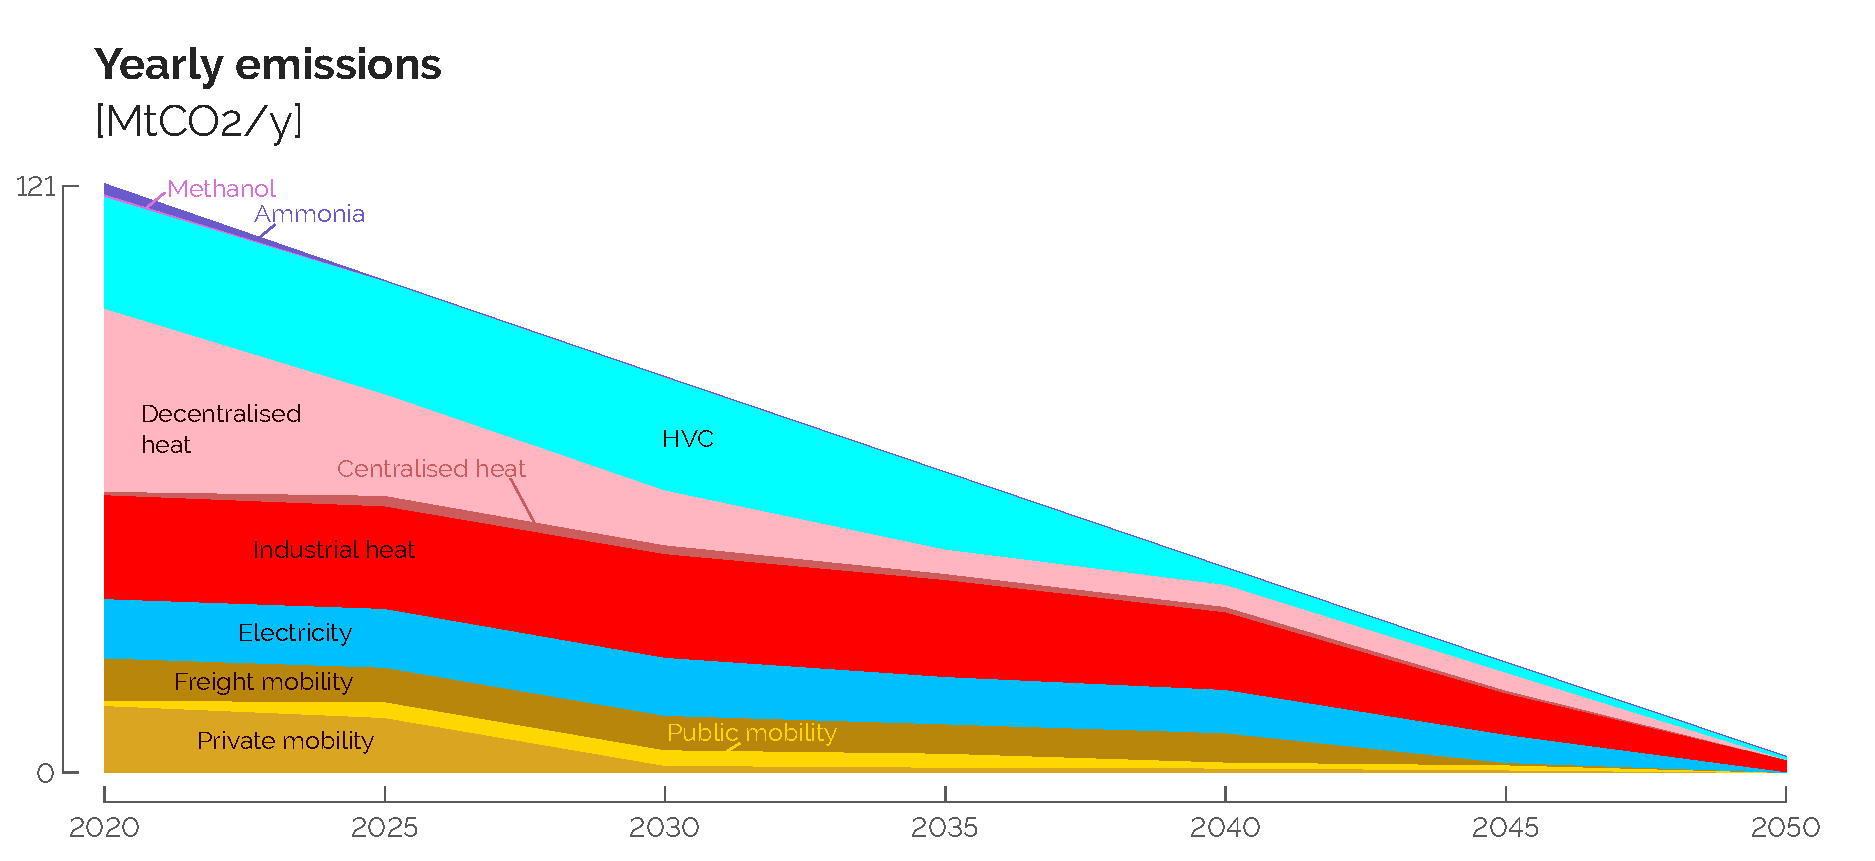
\includegraphics[width=\textwidth]{Gwp_per_sector.pdf}
\caption{Energy sectors have different speed to reduce \gls{GHG} emissions over the transition. The system uses all the allowed \gls{GHG} prescribed by the linear decrease from the emissions in 2020 until carbon-neutrality in 2050.}
\label{fig:pestd_ghg}
\end{figure}

The defossilisation of the different sectors are not performed at the same rate. The non-energy demand of methanol and ammonia are substituted by electrofuels. These are the first use of electrofuels as  e-ammonia is the cheapest electrofuel thanks to the high maturity of the Haber-Bosch process. The decentralised heat and mobility sectors are also dropping first. This is a combination of efficiency and substitution of fossil fuels with electricity. Efficiency comes mainly from district heating networks and electrical heat pumps for the heat sector, and public mobility and electric cars for the mobility sector. From 2040 onward, the decreases are mainly due to the substitution of the remaining fossil fuels by electrofuels as illustrated in Figure \ref{fig:pestd_primary_energy}.

Figure \ref{fig:pestd_primary_energy} shows the primary energy mix for the different representative years. The pathway verifies five trends: (i) reduction of primary energy thanks to energy efficiency; (ii) massive integration of endogenous renewable energies; (iii) importance of electrification; (iv) the usage of gas as the last fossil resource; and (v) the obligation to rely on renewable fuels to achieve carbon neutrality.

 \begin{figure}[!htbp]
\centering
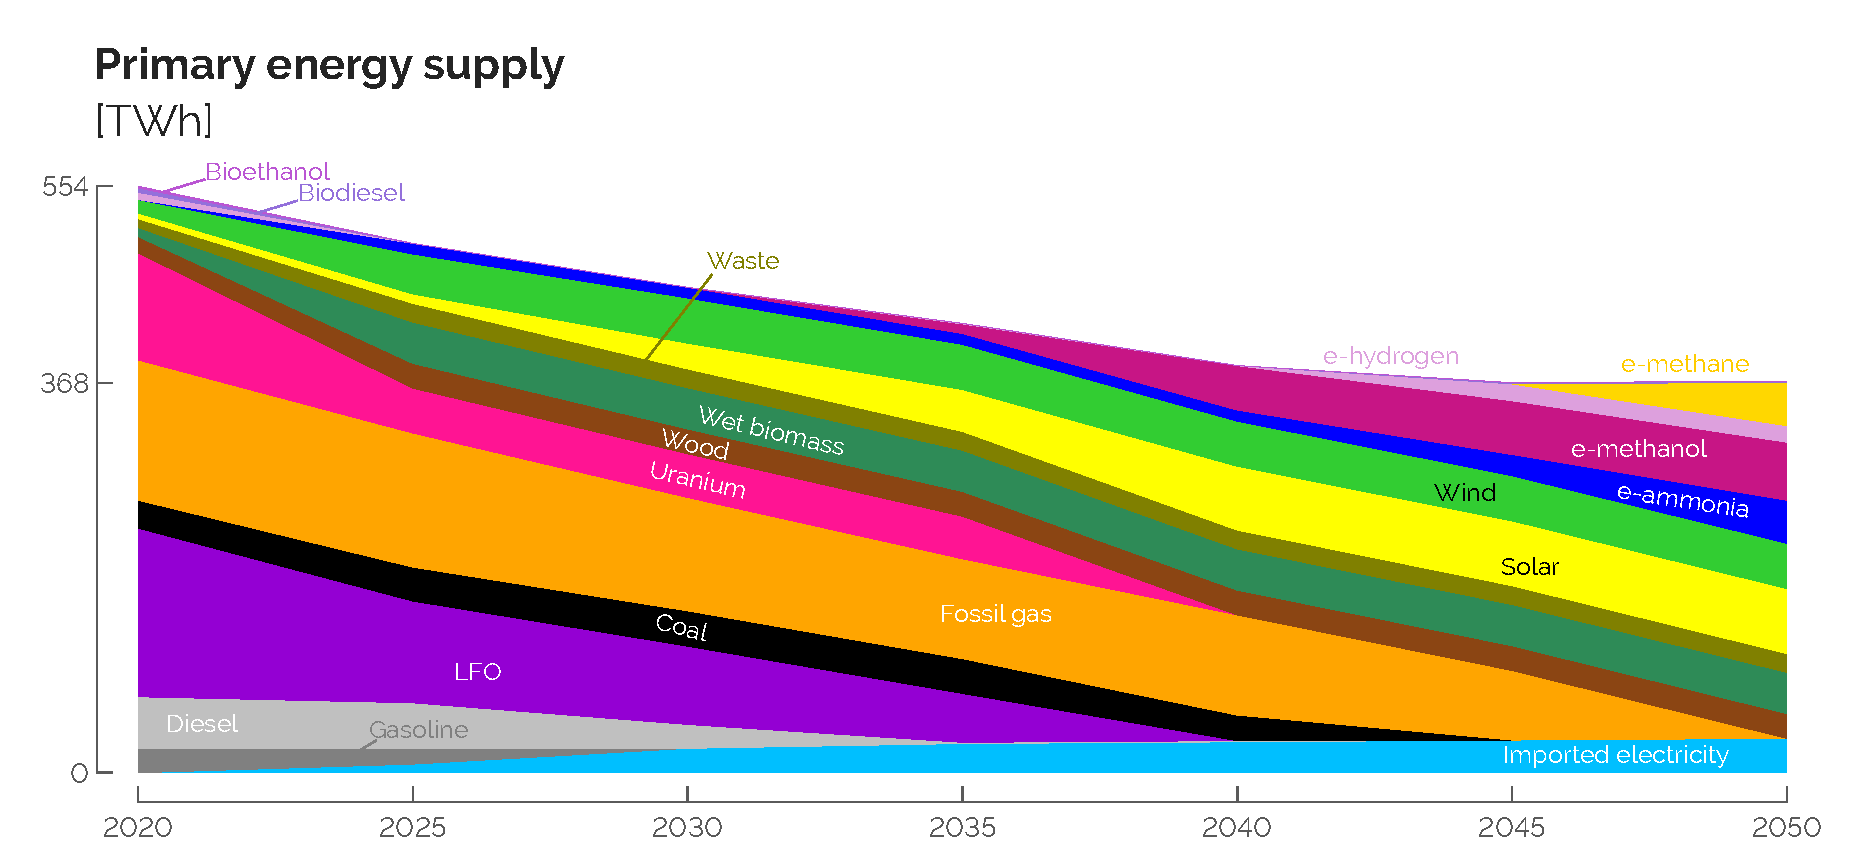
\includegraphics[width=\textwidth]{Resources.pdf}
\caption{Primary energy emitting \gls{GHG} (below Uranium) are reducing linearly with fossil gas remaining until 2045. A part of this energy is replaced by renewable ones and starting from 2040, a significant share of electrofuels. As end-use demands slightly increase (see Figure \ref{fig:cs_demands}), the drop represents energy efficiency (\ie providing the same services with less primary energy).}
\label{fig:pestd_primary_energy}
\end{figure}

The energy supply decreases from 554~TWh/y in 2020 down to 368~TWh/y in 2050 (\ie -34\%) whereas, in the meantime, the demands have increased by 19\%, on average. This drop of primary energy consumption reflects the penetration of efficient measures and technologies, such as the previously mentioned public mobility, \gls{DHN} or heat pumps. The results in 2050 are aligned with other studies, such as \citet{Devogelaer2013}\footnote{This study was ordered by the National Planning Bureau in 2013. Five scenarios are proposed.} and My2050\footnote{The Climate Change Service of the Federal Public Service Health launched an initiative in 2012 entitled `\emph{Low Carbon Belgium by 2050}'. This initiative resulted in a report and a calculator in 2013 \cite{Cornet2013}. The Belgian calculator has been improved since then into a recent expert version called \textbf{My2050} \cite{My2050}. From this study, the results of two scenarios will be used: one based on an optimistic evolution of technologies (Technology), and one focusing on an increased dependence on neighbouring countries (EU integration).} \cite{My2050} which estimates respectively a range of 305-417 TWh/y and 307-364~TWh/y for their central scenarios. 

The first fossil energy to phase out is gasoline, which is exclusively used for private cars. Indeed, private mobility is partially replaced by public one\footnote{Given the major role played by private cars in the Belgian passenger mobility nowadays (\ie around 80\% \cite{BFP_mob}), public transport (\eg tramways, buses and trains) is assumed to be able to supply only half of it.}; and the cars are switching from gasoline and diesel to electricity. Then, diesel and \gls{LFO} are decreasing. As diesel is used for trucks and buses mobility, it is harder to phase out compared to gasoline exclusively burned in cars. The first drop of \gls{LFO} reflects the switch from oil boilers to other technologies: heat pumps and gas cogeneration mainly. Then, it is mainly used for the production of \gls{HVC}, this reflects that \gls{HVC} is a feedstock hard to defossilise. Finally, coal is kept mainly for industrial usage because it is a cheap fossil fuel (mainly for industrial usage). To phase it out beforehand, a penalty mechanism, such as a carbon tax, would be required, or its strict ban should be put in place. The last fossil energy present in the system is fossil gas, used for the production of electricity and heat, through cogeneration mainly. Indeed, gas plays a key role to balance the intermittency of solar and wind.

The consumption of uranium declines in 2025, dropping to 2 GW, primarily due to the political framework aimed at phasing out nuclear energy \cite{nuclear_2035}. In the initial stages, significant deployment of endogenous energies takes place. This includes the utilization of wood, wet biomass, and wind energy, followed by the introduction of solar energy. However, solar energy is not fully deployed during this period due to higher integration costs. Starting from 2025, the importation of electrofuels begins, although their significant utilisation is observed from 2035 onwards. Initially, these fuels are predominantly employed as feedstocks in non-energy sectors. From 2040, e-methanol is additionally utilised for the production of High-Value Chemicals (HVCs), e-hydrogen is employed for mobility purposes, and both e-methane and e-ammonia are used for electricity generation through gas \gls{CHP} and ammonia-based \gls{CCGT} plants (see Figure \ref{fig:ELEC_tech_cap}).

In 2020, Belgium has been a net-exporter of electricity, however with the shut-down of nuclear power plants and the increase of electricity consumption, Belgium will become a net importer of electricity. These imports reach their maximal allowed capacity by 2035 (i.e. 30\% of electricity end use). This strong dependence on imported electricity illustrates the need for balancing intermittent renewables without relying on fossil fuels.

\subsection{Electricity sector: Capacities and yearly balance}
\label{subsubsec:elec_sector}
To better understand the electricity sector, the installed production capacities are given in Figure \ref{fig:ELEC_tech_cap}, while the supply-demand yearly balance is illustrated in Figure \ref{fig:ELEC_layer}.

\begin{figure}[!htbp]
     \centering
         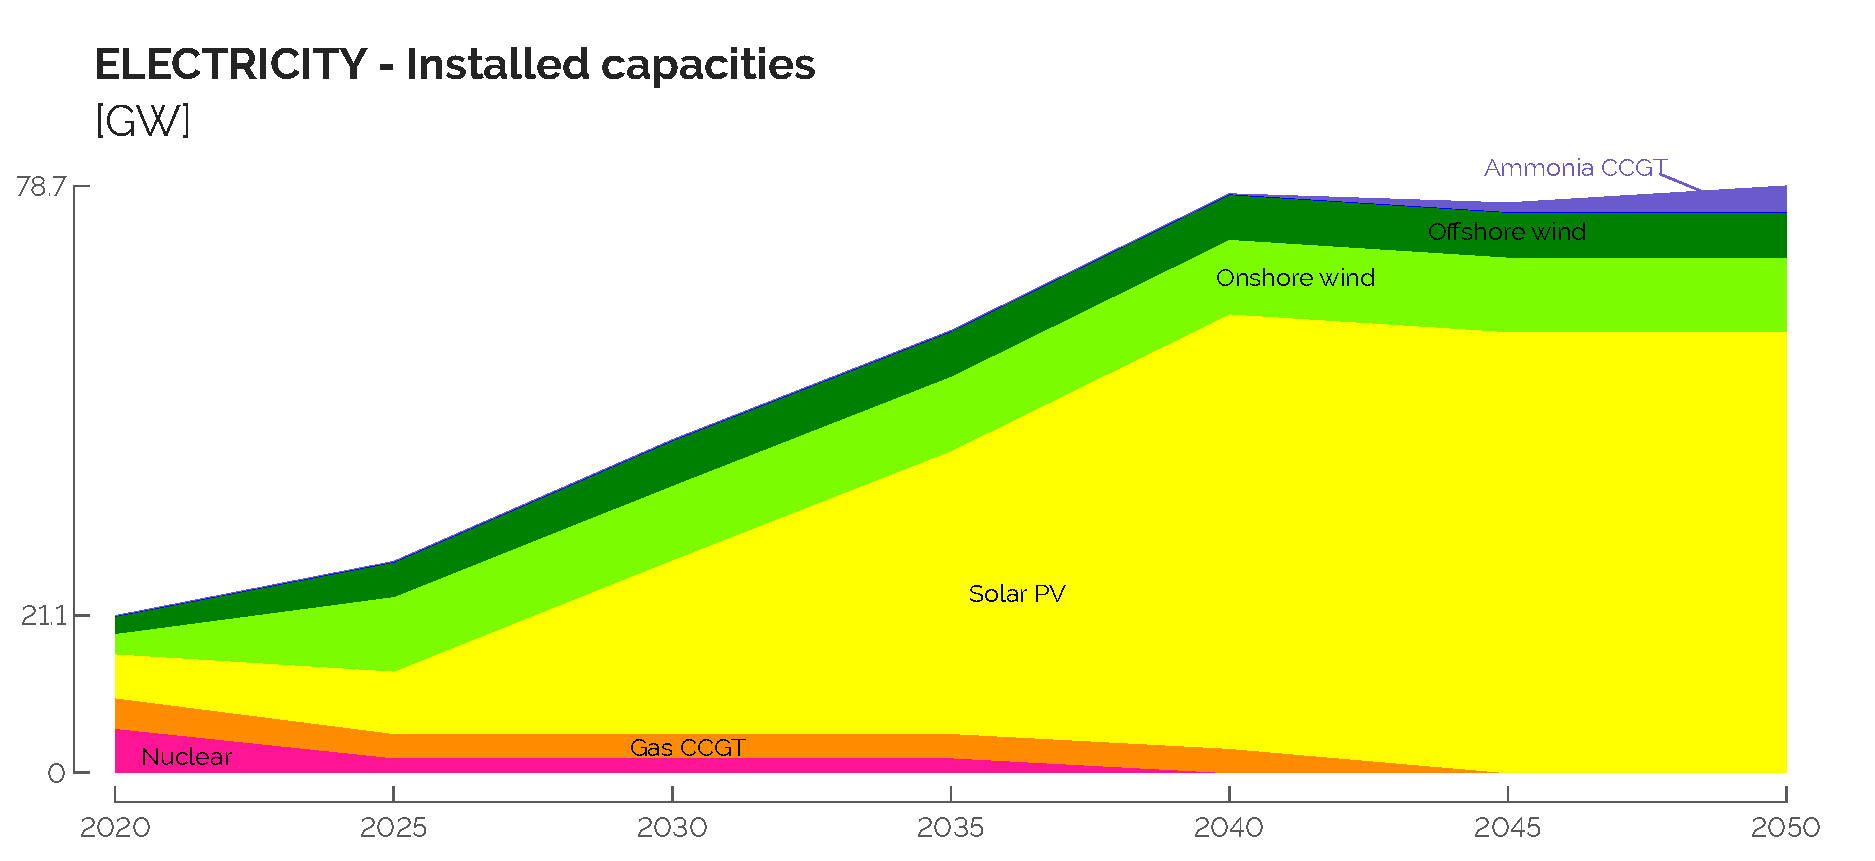
\includegraphics[width=\textwidth]{ELEC_tech_cap.pdf}
         \caption{The electrical production capacity will experience  massive expansion of wind turbines (onshore and then offshore) and a soaring installed capacity of \gls{PV}. Ammonia \gls{CCGT} are installed at the end of the transition to provide a flexible capacity as gas \gls{CCGT} are phased out.}
         \label{fig:ELEC_tech_cap}
\end{figure}


\begin{figure}[!htbp]
     \centering
         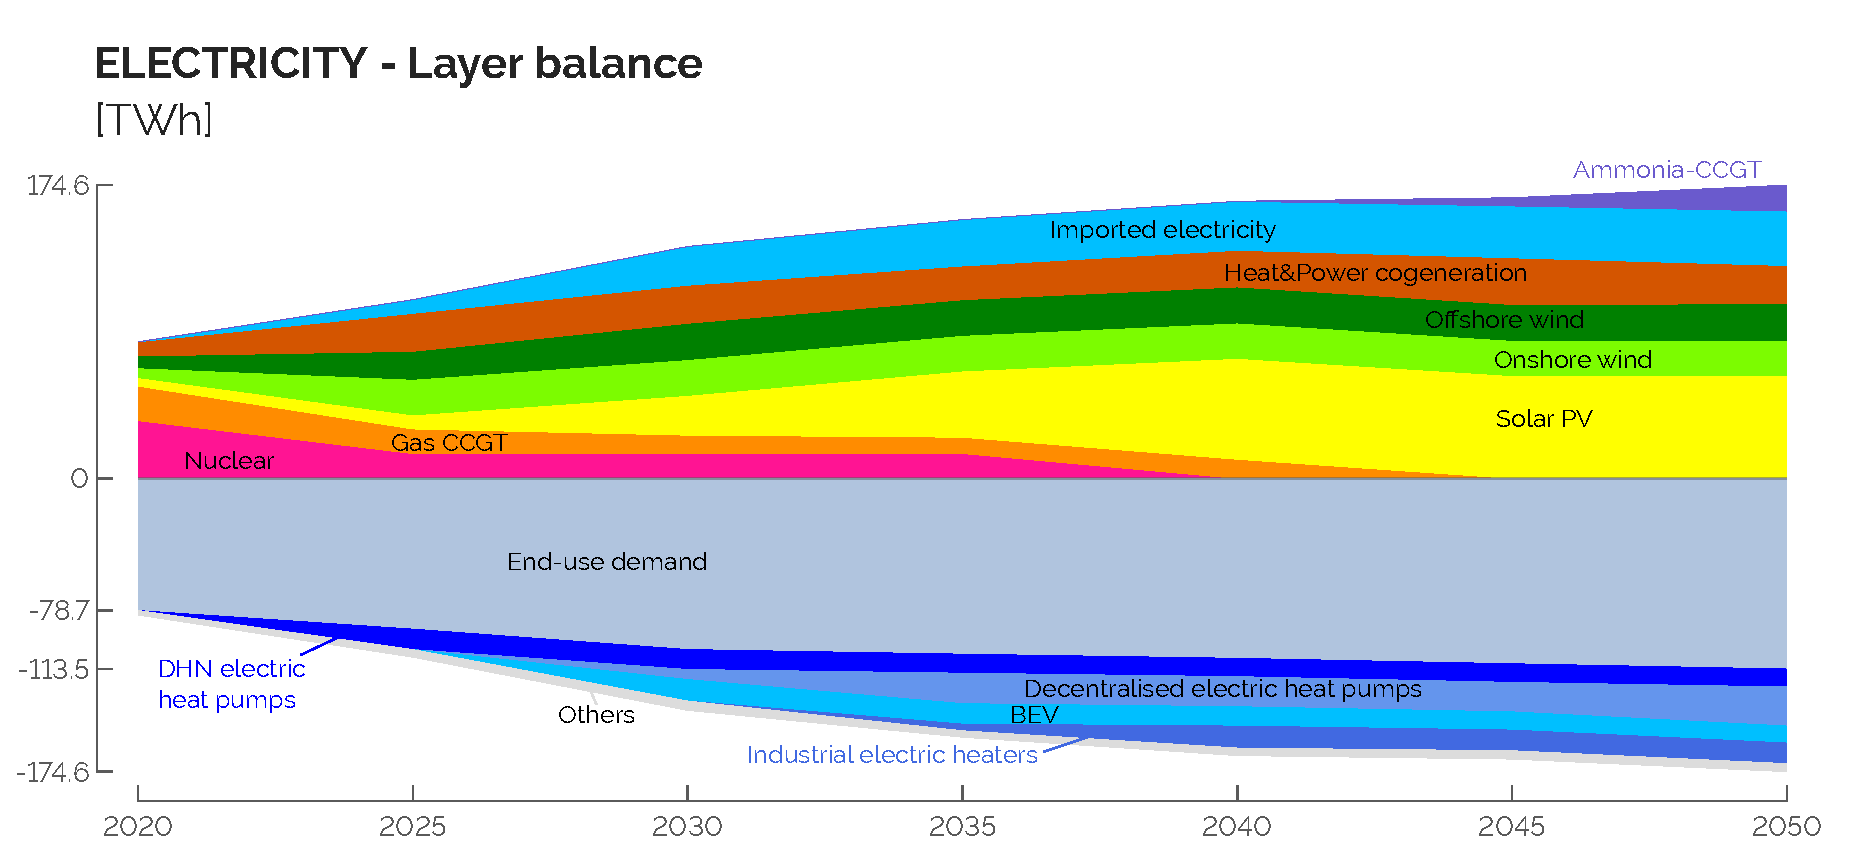
\includegraphics[width=\textwidth]{ELEC_layer.pdf}
         \caption{The electricity supply (positive values) will remain a mix of different technologies where backup is first mainly provided by gas-\gls{CCGT} and then imported electricity, heat and power cogeneration and later ammonia-\gls{CCGT}. The electricity demand (negative values) is led by the electricity end-use demand, but the share used to electrify heat (heat pumps), vehicles (cars, trains, trams, ...) and industrial heaters drastically increase. This enables a flexible demand that can facilitate the integration of intermittent renewables.}
         \label{fig:ELEC_layer}
\end{figure}

As introduced in the primary energy analysis (see Figure \ref{fig:pestd_primary_energy}), renewable capacities soar. By 2050, wind and solar technologies deployments are 60~GW of \gls{PV}, 10~GW of onshore wind turbines and 6~GW of offshore wind turbines. To compensate the intermittency, the system relies on imported electricity, gas \gls{CCGT}, sector coupling and storage. As an illustration, in 2050, 176.8~TWh of electricity transit on the grid which includes 32.4~TWh of electricity imported and 15.4~TWh of electricity from \gls{CCGT}. This result is aligned with other studies that estimates different ranges: 180-310 TWh/y \cite{Devogelaer2013}, 126-140~TWh/y \cite{My2050} and in a more recent study 
%\footnote{The EnergyVille consortium, made of belgian universities and research institutes, applied the TIMES-BE model to the case of Belgium to assess the energy transition pathways \cite{PATHS2050}. In this study, three scenarios are proposed: electrification, clean molecules and reference (called central in their report). They all reach carbon neutrality in 2050. The first allows more power production with new nuclear plants and more offshore wind. The clean molecules allow the import of synthetic molecules at a lower costs and have a more limited access to cross-border CO\textsubscript{2} storage.} 
using the TIMES-BE model, 185-196~TWh/y \cite{PATHS2050}. Higher values from \citet{Devogelaer2013} illustrate an almost exclusively electrified energy system. The differences between the study ranges reflect the different assumptions in terms of renewable potentials and availability of nuclear energy. A general trend is that Belgium should maximise its use of endogenous renewable resources, which \citet{dubois2023multi} identified as a cheaper option than importing additional renewable energies from abroad. Demand management reflects the flexible use of electricity, mainly through heat pumps that uncouple the heat demand and the electricity consumption when combined with thermal storage. Gas \gls{CCGT} is also a useful asset to compensate intermittent renewables. However, its capacity remains the same as the one installed in 2020. These results are verifying an hourly adequacy of the power demand. Moreover, in a previous study by \citet{pavivcevic2022bidirectionnal}, the snapshot version of the model has been coupled with Dispa-SET, a dispatch optimisation model. Results showed that the backup capacity was underestimated by less than 20\% to respect reserve capacity, mainly due the lack of reserve capacity for grid stability.  

From 2025, the electricity mix has a strong renewable share that rises up to 60\% in 2050. The remaining 40\% are mainly gas (or ammonia) in \gls{CCGT} and cogeneration and imported electricity. From a demand perspective, the electrification first starts with \gls{DHN} heat pumps, then electric cars, then decentralised heat pumps and finally industrial heaters. The latter reflects the usage of cheap \gls{PV} production peaks. 

\subsection{Costs: Investments and operation}

In the following paragraphs, the results are analysed from an economic perspective to decipher the choices made by the model, as the overall cost of the transition is 1 004~b€\textsubscript{2015} split unequally among the sectors. 

Figure \ref{fig:pestd_cumul_inv} illustrates the cumulative investments made throughout the transition, amounting to a total of 377.8 b€\textsubscript{2015}. Initially, the infrastructure, transport, and electricity sectors each account for approximately one-third of the investments. The investments in infrastructure are primarily driven by the electricity grid and the \acrfull{DHN}, representing a combined investment of 73 b€\textsubscript{2015}. The electricity sector's investment is led by power plants, totalling 31.5 b€. Notably, the investment costs in the mobility sector are primarily attributed to private cars, constituting 71\% of the total. A rough estimation confirms the significant investment in cars, with an average of 500,000 vehicles registered annually in Belgium over the last decade \cite{febiac2021datadigest} and assuming an average cost of 20 k€ per car, the funds allocated to private cars amount to 10 b€ per year. This trend in private cars explains why the private mobility sector accounts for half of the investments required to achieve the transition by 2050. This finding aligns with other studies, such as \citet{Devogelaer2013}, which estimates cumulative investment expenditures of approximately 600 b€\textsubscript{2005} for the transport sector between 2013 and 2050, which confirms our conservative approach in the estimation.


As a comparison, the investments required to fully deploy the PV and wind potentials from 2020 to 2050 amount to 74.4 b€\textsubscript{2015}, with an additional 22.2 b€\textsubscript{2015} allocated to reinforce the grid. The electrification of the heating sectors necessitates investments of 29.2 b€\textsubscript{2015}, including 6.5 b€\textsubscript{2015} for the deployment of the \gls{DHN} infrastructure. Storage investments, primarily focused on \gls{DHN} seasonal storage, amount to 3.6 b€\textsubscript{2015}. Apart from the investment required to replace all private vehicles (accounting for 44\% of the overall investments), the remaining sectors represent a total of 212 b€\textsubscript{2015}. To mitigate the cost of the transition, My2050 suggests deploying a fleet of no more than one million vehicles and implementing a car sharing system, distinct from car-pooling, as an inevitable measure \cite{My2050}.

\begin{figure}[!htbp]
\centering
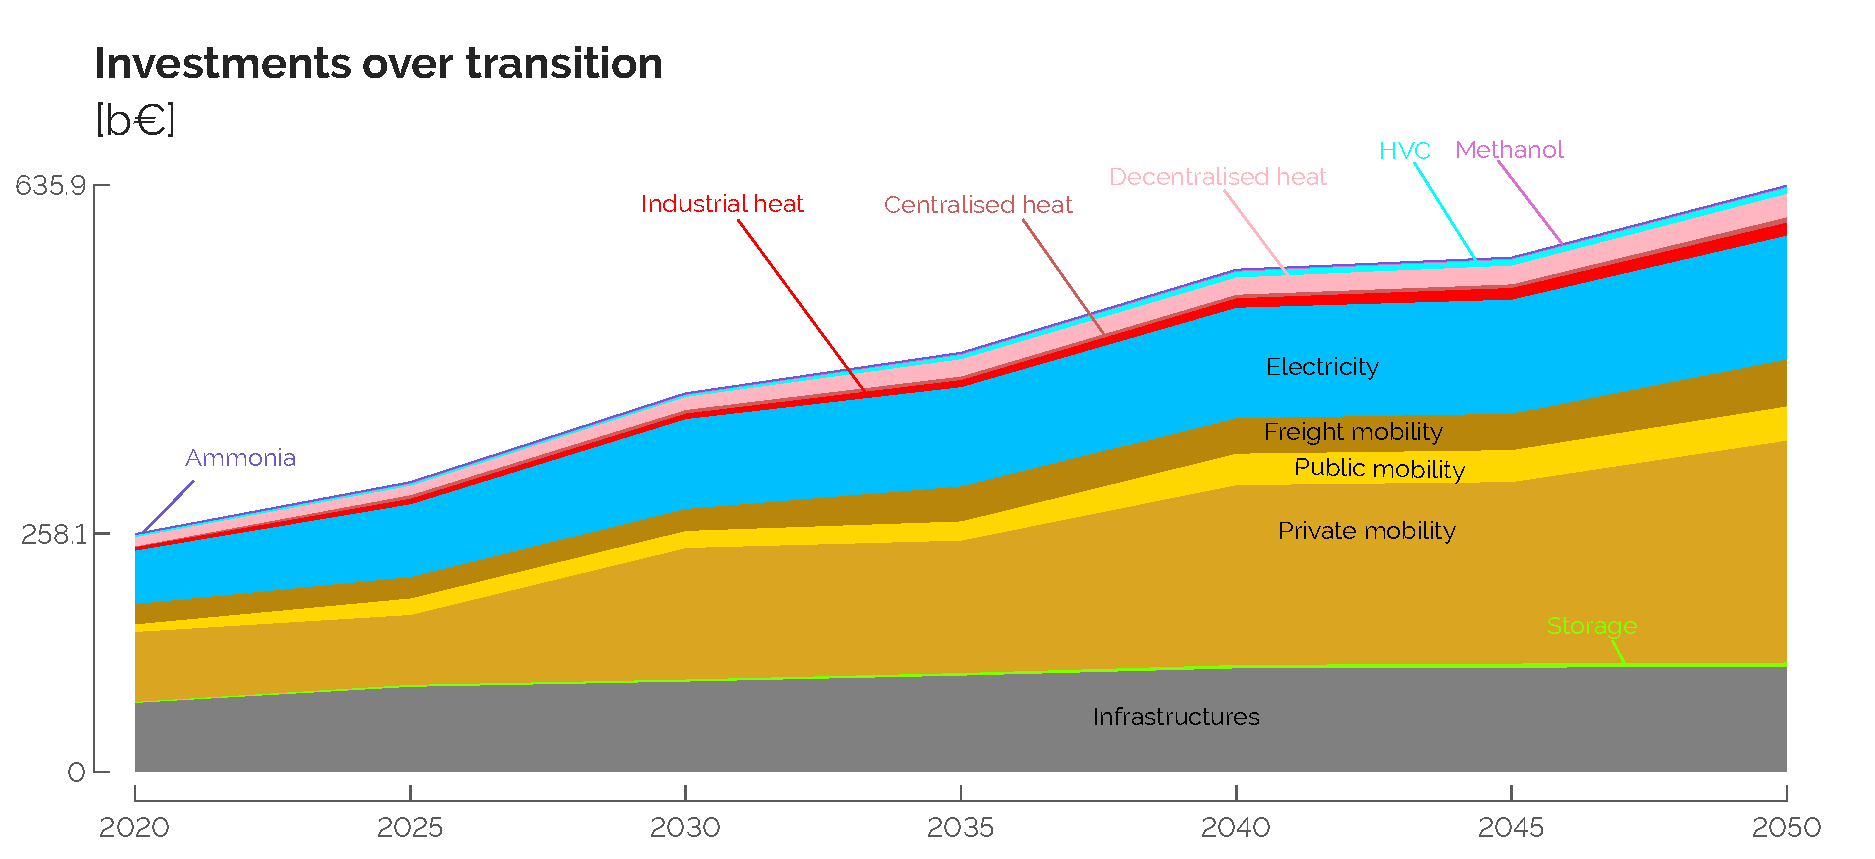
\includegraphics[width=\textwidth]{Investment_transition.pdf}
\caption{The cumulative investments over the transition is unequally spread between the sectors. The energy system in 2020 is imposed to the existing energy system and its expenses are split in three main categories: mobility (mainly vehicles), infrastructure (mainly grids) and electricity (mainly thermal power plants). The investments required during the transition represents 150\% the initial investment and mainly in the same three sectors. }
\label{fig:pestd_cumul_inv}
\end{figure}

A part of the investment will be recovered at the end of the transition based on the remaining lifespan of the technology after 2050. Figure \ref{fig:pestd_inv_return} illustrates the salvage value by sectors, calculated according to Eq. (\ref{eq:salvage}). Out of the 114.4~b€\textsubscript{2015} of investments in the infrastructure (\ie mostly power grid and gas network), 55.9\% remain available after 2050, due to their long lifetime. On the contrary, private mobility has a lower salvage value due to a major drop within the first four years and an average lifetime below 10 years \cite{febiac2021datadigest}. 
% Consequently, out the 240.5~b€\textsubscript{2015}, including the initial investment of 75.7~b€\textsubscript{2015}, only 13.9\% would remain available after 2050.


\begin{figure}[!htbp]
\centering
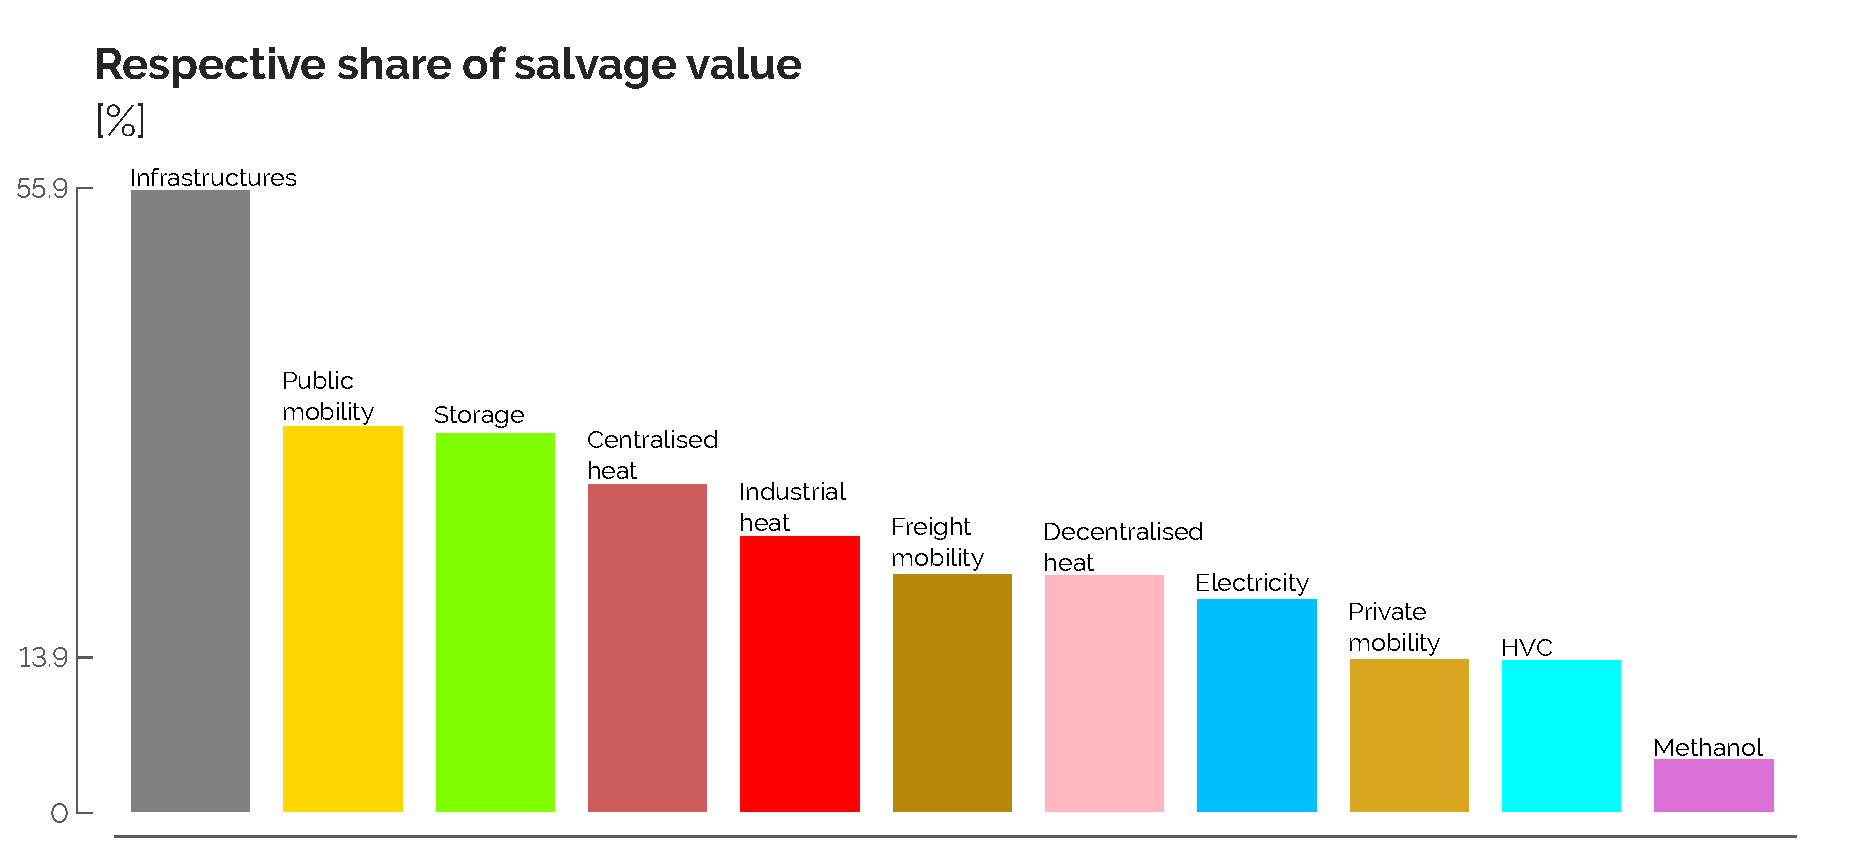
\includegraphics[width=\textwidth]{Investment_return.pdf}
\caption{By the end of the transition (\ie in 2050), the ratio between the salvage value and its cumulative investment, per sector, is unequal. Investments in infrastructures, public mobility, storage and other long-lifetime technologies experience an important salvage value, at the contrary, investments in private mobility will not be recovered as vehicles have a short lifetime. All together, these salvage values represent 160.1 b€\textsubscript{2015}, 25\% of the cumulative investment costs in 2050.}
\label{fig:pestd_inv_return}
\end{figure}

In addition to investment decisions, the \acrfull{OPEX}, which accounts for resource utilisation and technology maintenance, are significant. Figure \ref{fig:pestd_cumul_op} shows the yearly system cost for each sector except the \gls{OPEX} related to resources that are grouped together. The latter dominates the \gls{OPEX}, with a significant share of non-renewable resources (\ie 63.6\% in 2020) until 2040, followed by a steep increase in the share of renewable resources (\ie 66.2\% in 2050). The substantial reliance on non-renewable resources reflects the prevalent use of fossil fuels in our current energy system. The high cost-share of non-renewable fuels underscores the economic challenges of simply substituting fossil fuels with renewables, particularly evident when emphasizing that electrofuels are 2-3 times more expensive. Maintenance expenses in the private mobility sector rank second in terms of expenditure. On the other hand, maintenance expenses in other sectors are relatively small compared to the aforementioned sectors.

\begin{figure}[!htbp] %@GL: check that text is aligned with new figure.
\centering
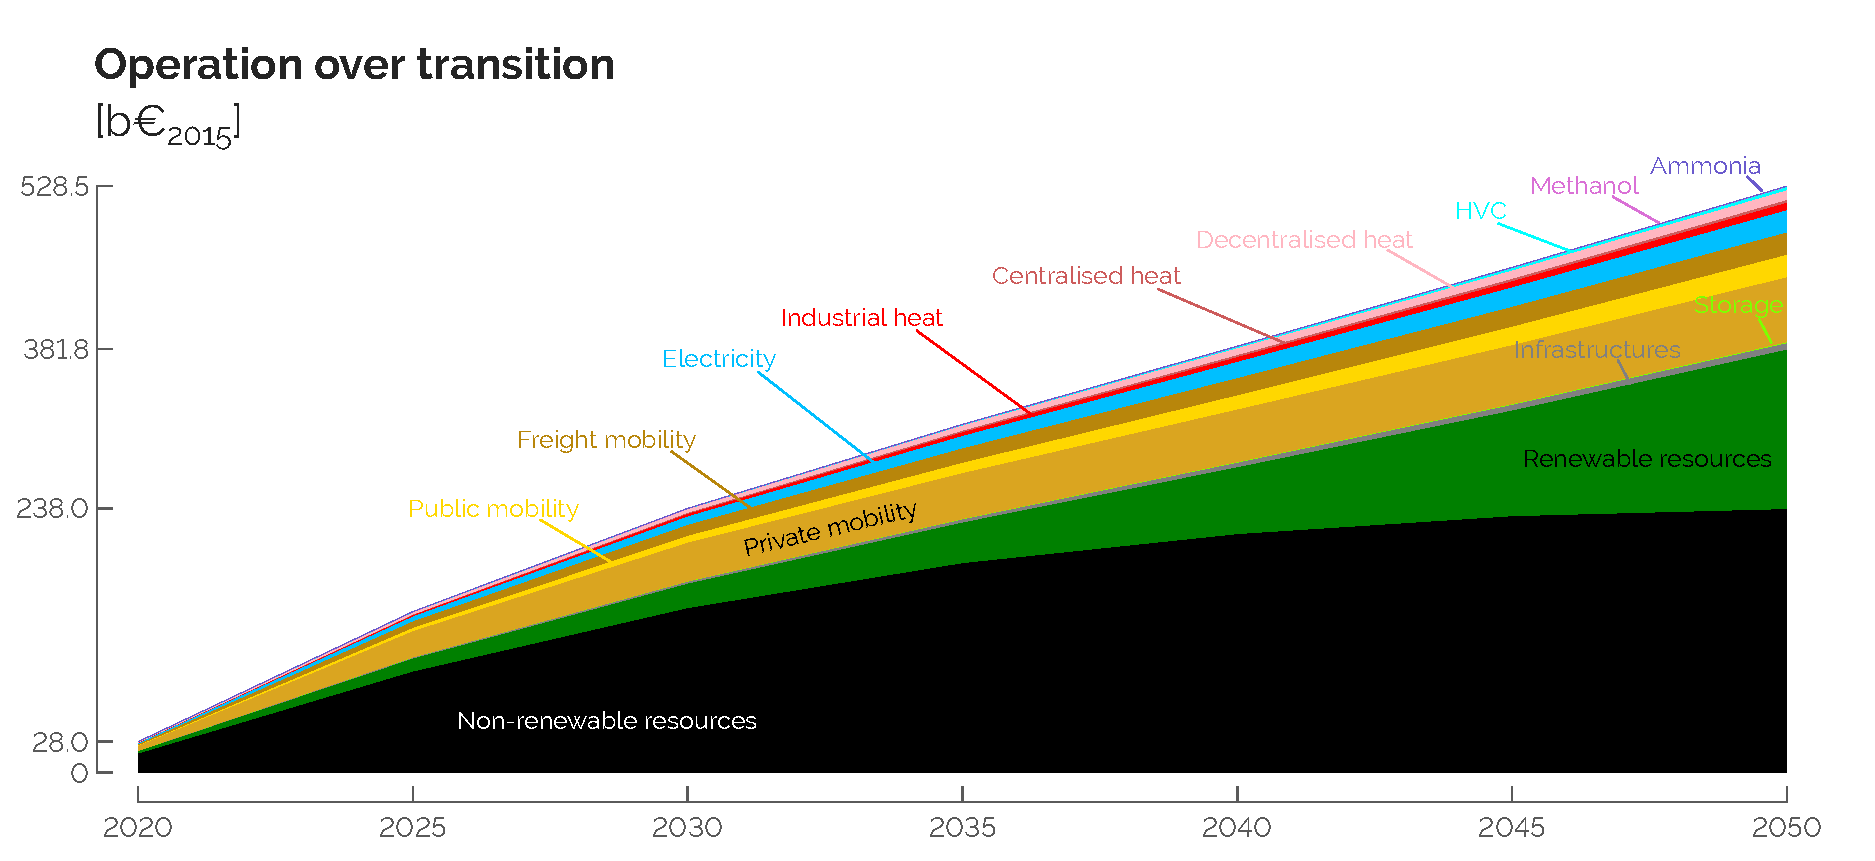
\includegraphics[width=\textwidth]{Operation_transition.pdf}
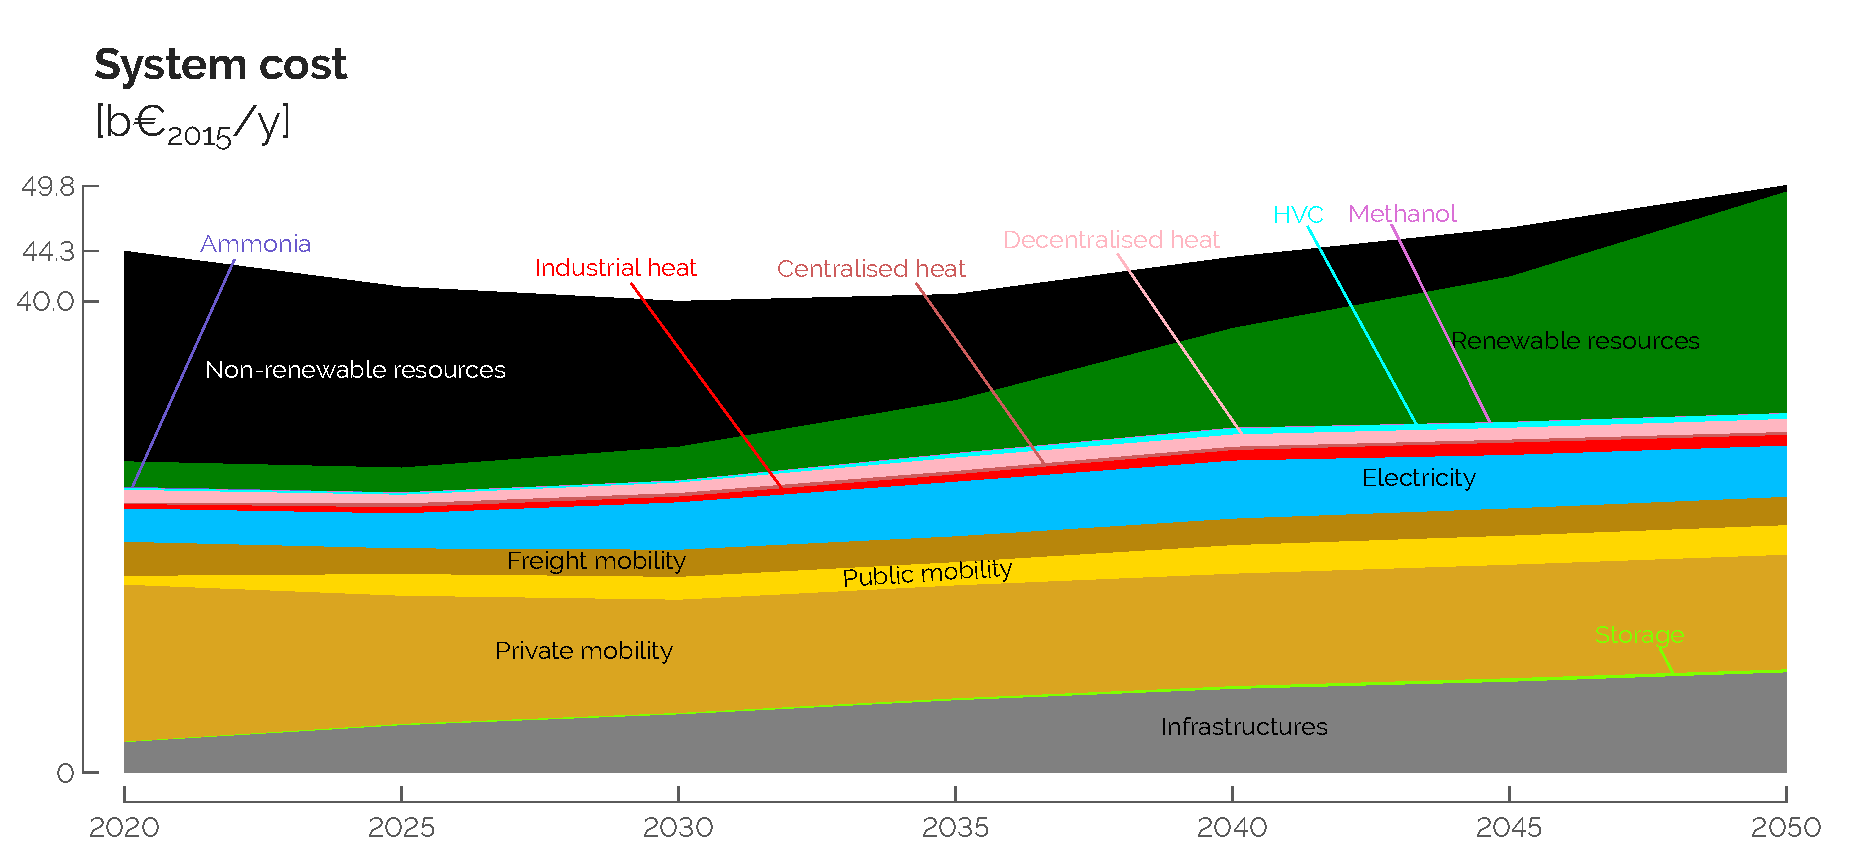
\includegraphics[width=\textwidth]{System_cost.pdf}
\caption{The yearly system cost shows the shift from non-renewable to renewable resources (mainly electrofuels). Operation cost and maintenance represents almost 50\% of the expenses.}
\label{fig:pestd_cumul_op}
\end{figure}

The annualised cost of the energy system in 2020 is estimated to 44.3~b€/y and increases by 5.5~b€/y to reach 49.8~b€/y by 2050. The work of \citet{My2050} estimates the annualised cost in 2050 between 63 and 82~b€/y, while the other studies just indicate the cost increase compared to 2015 (+11.7 to +21) \citep{Devogelaer2013,PATHS2050}. The differences come from the scope of the energy system: as an example \citet{My2050} also account for the agriculture sector. These differences highlight the difficulty to compare different studies due to difference of scope and partial availability of used data. Overall, comparing with existing studies shows the consistency of the results provided by EnergyScope Pathway.

\section{Myopic versus perfect foresight pathway optimisation}
\label{app:my_vs_pf}
This section aims at digging more into the details of the differences observed between the myopic approaches and the reference case (\ie hourly perfect foresight model).

\begin{table}[htbp]
\caption{Exhaustive general comparison between the two different foresight approaches: Perfect foresight (PF) and Myopic (MY). Differences with the reference case (PF) below 1\% are not shown ($\simeq$) and ones above 10\% are in bold.}
\label{tab:PF_MY}
\begin{minipage}{\textwidth}
\centering
\resizebox{\textwidth}{!}{
\begin{tabular}{l l r r c}
\toprule
& & {\thead{\textbf{PF}}} & {\thead{\textbf{MY}}} & Units \\
\midrule
Computational time\footnote{\label{foot:comp_time}These computational times were reached on a 2.4GHz 4-core machine.} & & 830 & \textbf{373} & s \\
\midrule
\multirow{4}{*}{Costs in 2050}
& Total transition\footnote{\label{foot:transition_cost}As detailed in \autoref{eq:obj_func_v2}, the transition cost is the sum of the cumulative opex and capex, salvage value being deduced.} & 1004 & $\simeq$ & b€\textsubscript{2015}\\
& Cumulative opex & 528 & $\simeq$  & b€\textsubscript{2015}\\
& Cumulative capex & 636 & $\simeq$ & b€\textsubscript{2015}\\
& Salvage value & 160 & -1\% & b€\textsubscript{2015}\\
\midrule
\multirow{5}{*}{Primary energy mix in 2050} & Total & 368.0 & $\simeq$ & TWh/y\\
 & e-hydrogen & 15.6 & $\simeq$ & TWh/y\\
 & e-methane & 41.0 & +6\% & TWh/y\\
 & e-methanol & 54.8 & $\simeq$ & TWh/y\\
 & e-ammonia & 40.7 & -10\% & TWh/y\\

 \midrule
 \multirow{3}{*}{Electrification in 2050\footnote{\label{foot:share_elec}The electrification of the other sectors (\ie centralised heat (100\%-heat pump), private (100\%-\gls{BEV}), public mobility (80\%-train and tramway), freight mobility (25\%-train) and non-energy demand (0\%)) are identical between the three approaches and are, therefore, not presented in the table.}} & System\footnote{\label{foot:system_elec}The electrification of the system is computed as the difference between the total production of electricity and the end-use demand of electricity.} & 63.3 & $\simeq$ & TWh$_{\text{e}}$\\ 
 & Industrial heat\footnote{\label{foot:heat_elec}The electrification of the industrial and decentralised heating sectors are expressed in terms of thermal energy (TWh$_{\text{th}}$) provided by electrified processes, respectively industrial resistors and decentralised electric heat pumps.} & 12.3 & -7\% & TWh$_{\text{th}}$\\
 & Decentralised heat\footref{foot:heat_elec} & 73.9 & $\simeq$ & TWh$_{\text{th}}$\\
  \midrule
\multirow{3}{*}{Year of full VRES-deployment} & PV & 2045 & \textbf{2040} & -\\
 & Wind-offshore & 2030 & \textbf{2025} & -\\
 & Wind-onshore & 2025 & 2025 & -\\
\bottomrule
\end{tabular}
}
\end{minipage}
\end{table}




Similarly to \citet{nerini2017myopic}, Figure \ref{fig:my_pestd_total_cost_cum_diff} shows that myopic optimisation ends up with a slightly more expensive energy transition by 2050 (\ie +3.2~b€$_{2015}$), compared to the perfect foresight, despite the savings done at the early stages. Even though this over-cost is negligible compared to the overall cost of the transition (\ie $\sim$1000~b€$_{2015}$), this is explained by the early investments in renewable technologies (\ie PVs and wind turbines) boosted by the significant salvage value retrieved from investing in the consequent reinforcement of the grid. 

Figure \ref{fig:my_pestd_inv_return_area} highlights this as infrastructures and the electricity-technologies account respectively for 83.2 and 61.2~b€\textsubscript{2015} in 2030 whereas the overall cumulative investments, so far, are 421.3~b€\textsubscript{2015}. The significant lifetime (\eg 80 years) and investment cost (\ie 368M€/GW$_\text{VRES}$ \cite{readthedocs_pathway}) of the power grid, and, on a smaller scale, the district heating network, explain why the myopic optimisation opts for a higher investment in these infrastructures, at early stages. Similarly to what \citet{keppo2010short} observed in their studies, these early investments consequently lead to more investments, later in the transition, to renew technologies that have become too old before 2050: during the phase between 2045 and 2050, the myopic approach needs to invest in 9.2GW of PVs that have been installed 25 years before whereas the perfect foresight, by smoothing its investments over the entire transition, has to renew only 2.5GW of PVs. 

\begin{figure}[!htbp]
\centering
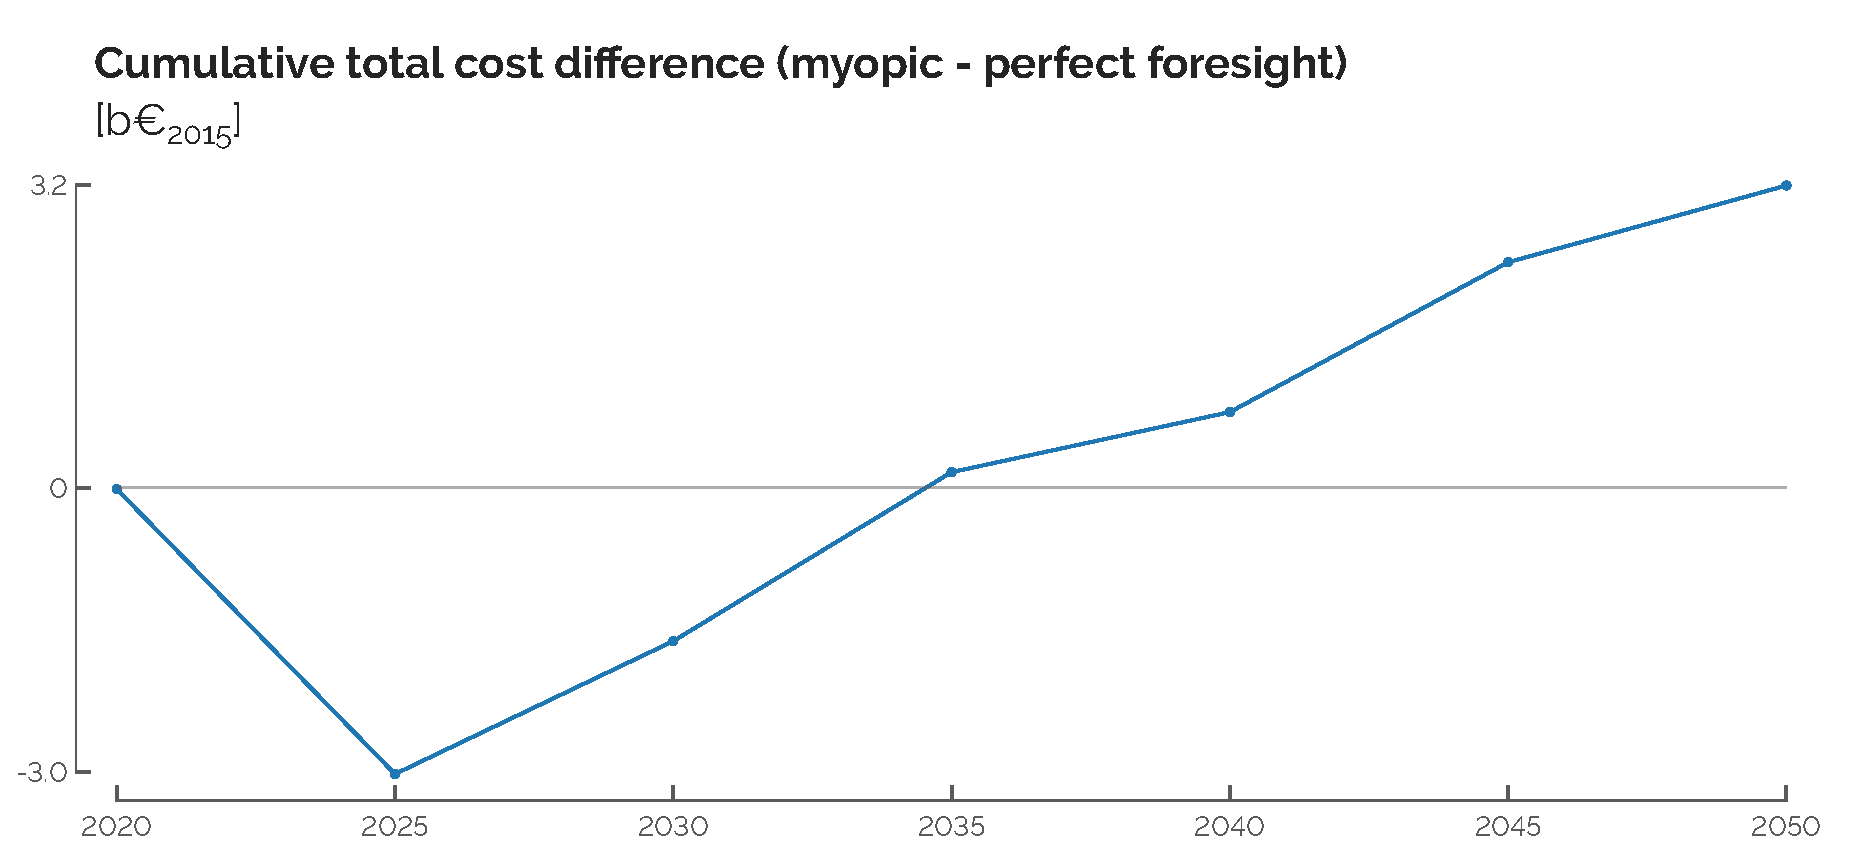
\includegraphics[width=\textwidth]{MY_cumulative_total_cost_diff.pdf}
\caption{Cumulative total cost (i.e. opex+capex-salvage value) difference between the myopic and perfect foresight (PF) approaches. Positive values mean that the myopic approach is higher than perfect foresight. Early savings of the myopic vision are overcompensated by late investments further on.}
\label{fig:my_pestd_total_cost_cum_diff}
\end{figure}

In 2050, the capacities installed in the different sectors, the design of the system in other words, are very similar between the two approaches. The passenger and freight mobility sectors are the same where differences smaller than 1GW are observed in other sectors. More interestingly, the myopic optimisation tends to postpone the decommissioning of capacities when the loss of salvage values at the end of an optimisation window would be bigger than the maintenance cost. For instance, in the myopic approach, 0.8GW of industrial coal boilers will remain installed in 2045 and 2050 or 3.6GW of naphtha-crackers to produce HVC in 2040, whereas these technologies are not used. This is comparable to the ``lock-ins" detailed in other studies \cite{heuberger2018impact,keppo2010short} where technologies installed at early stages of the transition remain in place.

Highlighted in Figure \ref{fig:my_pestd_res_cat_diff}, the earlier availability of renewable (and intermittent) electricity consequently accelerates the electrification of the other sectors. For instance, in 2035, 3.7GW (+75\%) more of industrial electric heaters to produce 5.1TWh/year (+130\%) of additional industrial heat. In the low-temperature heat sector, decentralised and centralised electric heat pumps capacities are, respectively, 2.2GW (+19\%) and 1GW (+8\%) higher for each of the representative years between 2030 and 2045, to produce, around 7.8TWh/year (+23\%) and 0.8TWh/year (+1\%), at the expense of other technologies such as gas heat pumps. Finally, public trains substitute from 2035 a higher share of the CNG-buses.

In general, due to the formulation of the salvage value (see Eq. \ref{eq:salvage}), the myopic approach is more techno-oriented as investing more in technologies is beneficial, especially at the early stages of the transition. Therefore, before converging to a similar energy mix in 2050, the myopic system relies more on local renewables (\eg solar and wind) than on importing renewable energy carriers (\eg e-ammonia, e-methanol, e-hydrogen or e-methane), see Figure \ref{fig:my_pestd_res_cat_diff}. In parallel, in the near term, the system relies on average more on conventional/non-renewable sources, like observed in other studies \cite{keppo2010short,nyqvist2005limited,hedenus2006induced}.

\begin{figure}[!htbp]
\centering
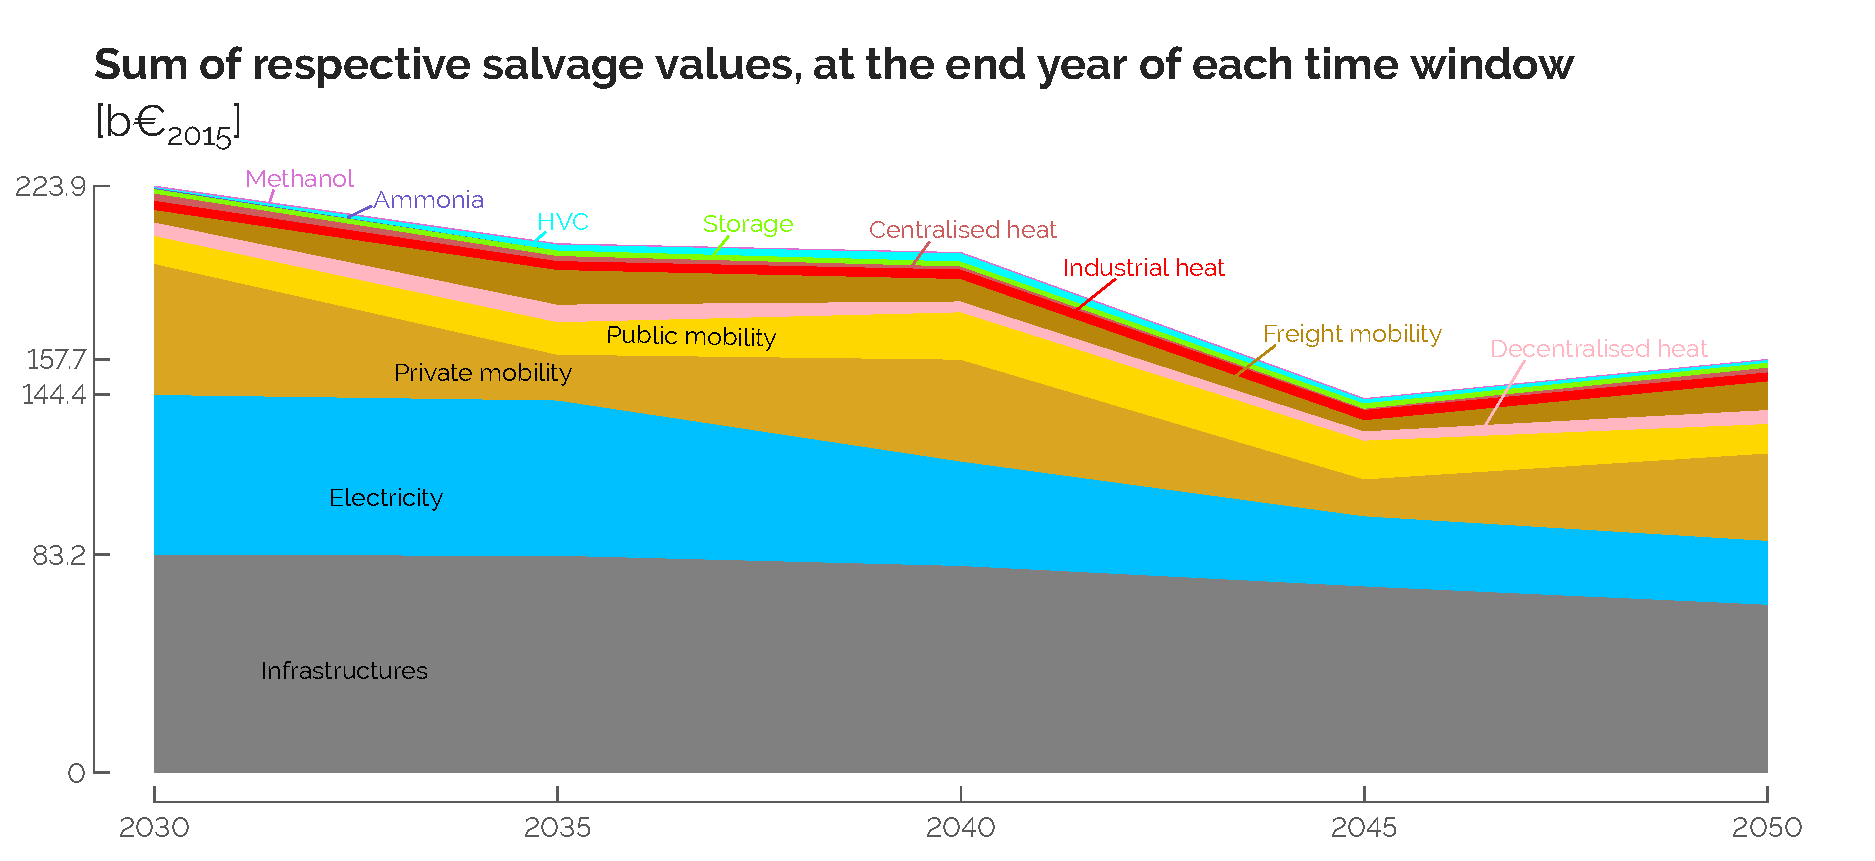
\includegraphics[width=\textwidth]{MY_investment_return_area.pdf}
\caption{Sum of the respective salvage value of each sector, per end year of each time window. All together, these salvage values represent 223.9~b€\textsubscript{2015}, 53\% of the cumulative investment costs in 2030, and 157.7~b€\textsubscript{2015}, 24\% of the cumulative investment costs in 2050.}
\label{fig:my_pestd_inv_return_area}
\end{figure}

 \begin{figure}[!htbp]
\centering
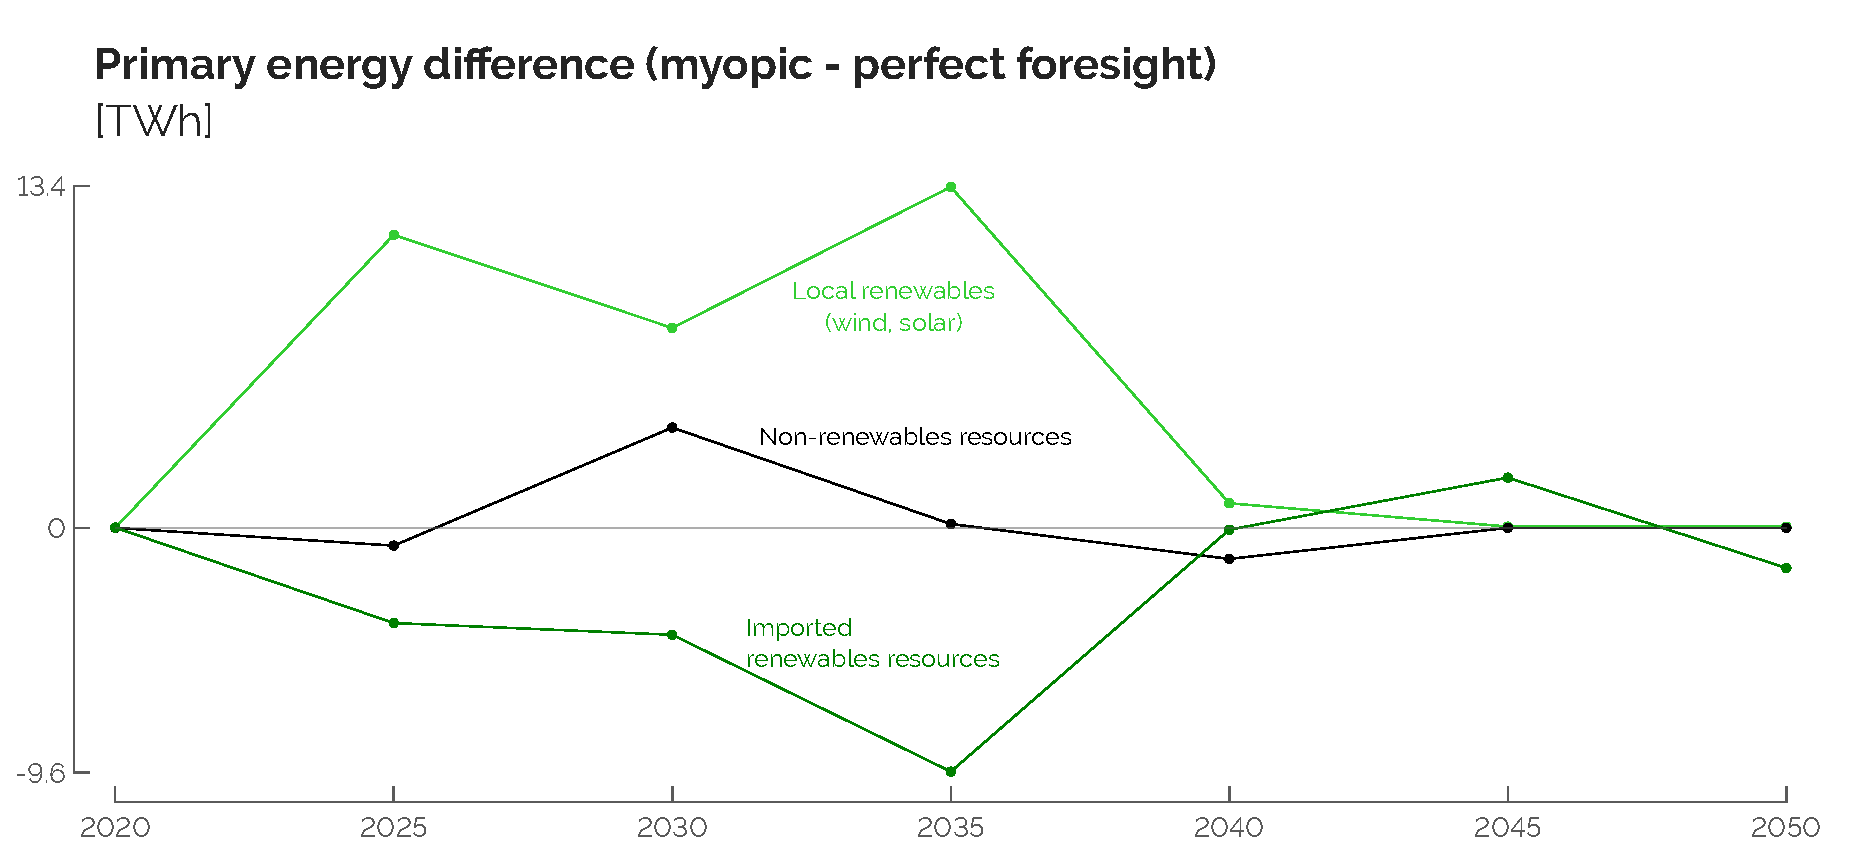
\includegraphics[width=\textwidth]{MY_resources_category_diff.pdf}
\caption{Primary energy resources difference between the myopic and perfect foresight (PF) approaches. Positive values mean that the myopic approach is higher than perfect foresight.}
\label{fig:my_pestd_res_cat_diff}
\end{figure}

\section{Assessment of different emissions-trajectories}
\label{app:CO2_trajectories}
This section compare results of the optimisation subject to different emissions-trajectories with the REF case where the emissions are constrained to decrease linearly from the level in 2020 to carbon-neutrality in 2050. The first comparison is done with the trajectory subject to respect the \ce{CO2}-budget prescribed in the \gls{RL}-based pathway optimisation, \ie 1.2\,Gt$_{\ce{CO2},\text{eq}}$ (Section \ref{sec:cs:CO2-budget}). Then, to assess the impact of the myopic approach on the optimisation of the transition, it is compared to perfect foresight results, alleviating the constraint on the emissions-trajectory.


\subsection{\ce{CO2}-budget versus linear decrease of emissions}
\label{app:CO2_budget}

\Cref{fig:app_CO2_REF_lin} shows the yearly emissions attributed for each sector in the REF case (\ie imposed \ce{CO2}-budget) and a case where the \ce{CO2}-trajectory is constrained instead. Interestingly, these two transition pathways end up in a similar carbon-neutral whole-energy system in 2050. The two main sectors that significantly reduce their emissions in the REF case are the production of \gls{HVC} and the high-temperature heat. In the former, this is linked to the extended use of oil products through naphtha-cracking. The latter is produced by industrial coal boilers for longer, until 2040. Overall, ending up to the same level of emissions in 2050, the REF case represents a 60\% reduction of the cumulative emissions compared to the linear decrease, for a 7.5\% more expensive transition.

\begin{figure}[htbp!]
\centering
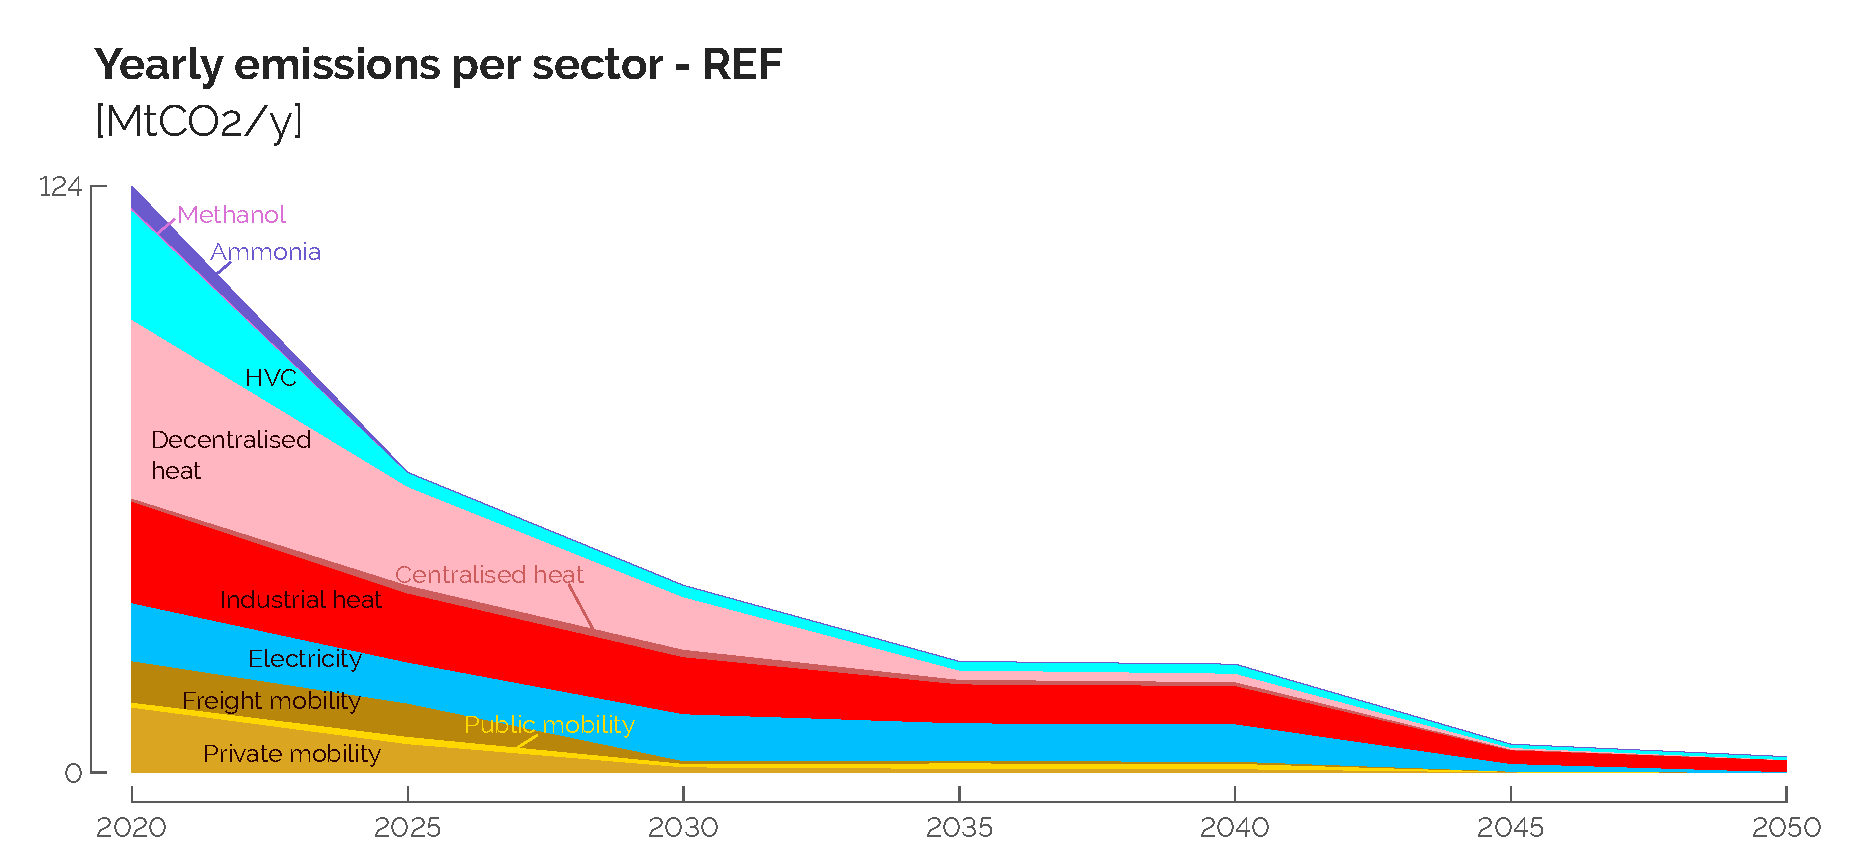
\includegraphics[width=0.49\textwidth]{GWP_per_sector_REF.pdf}
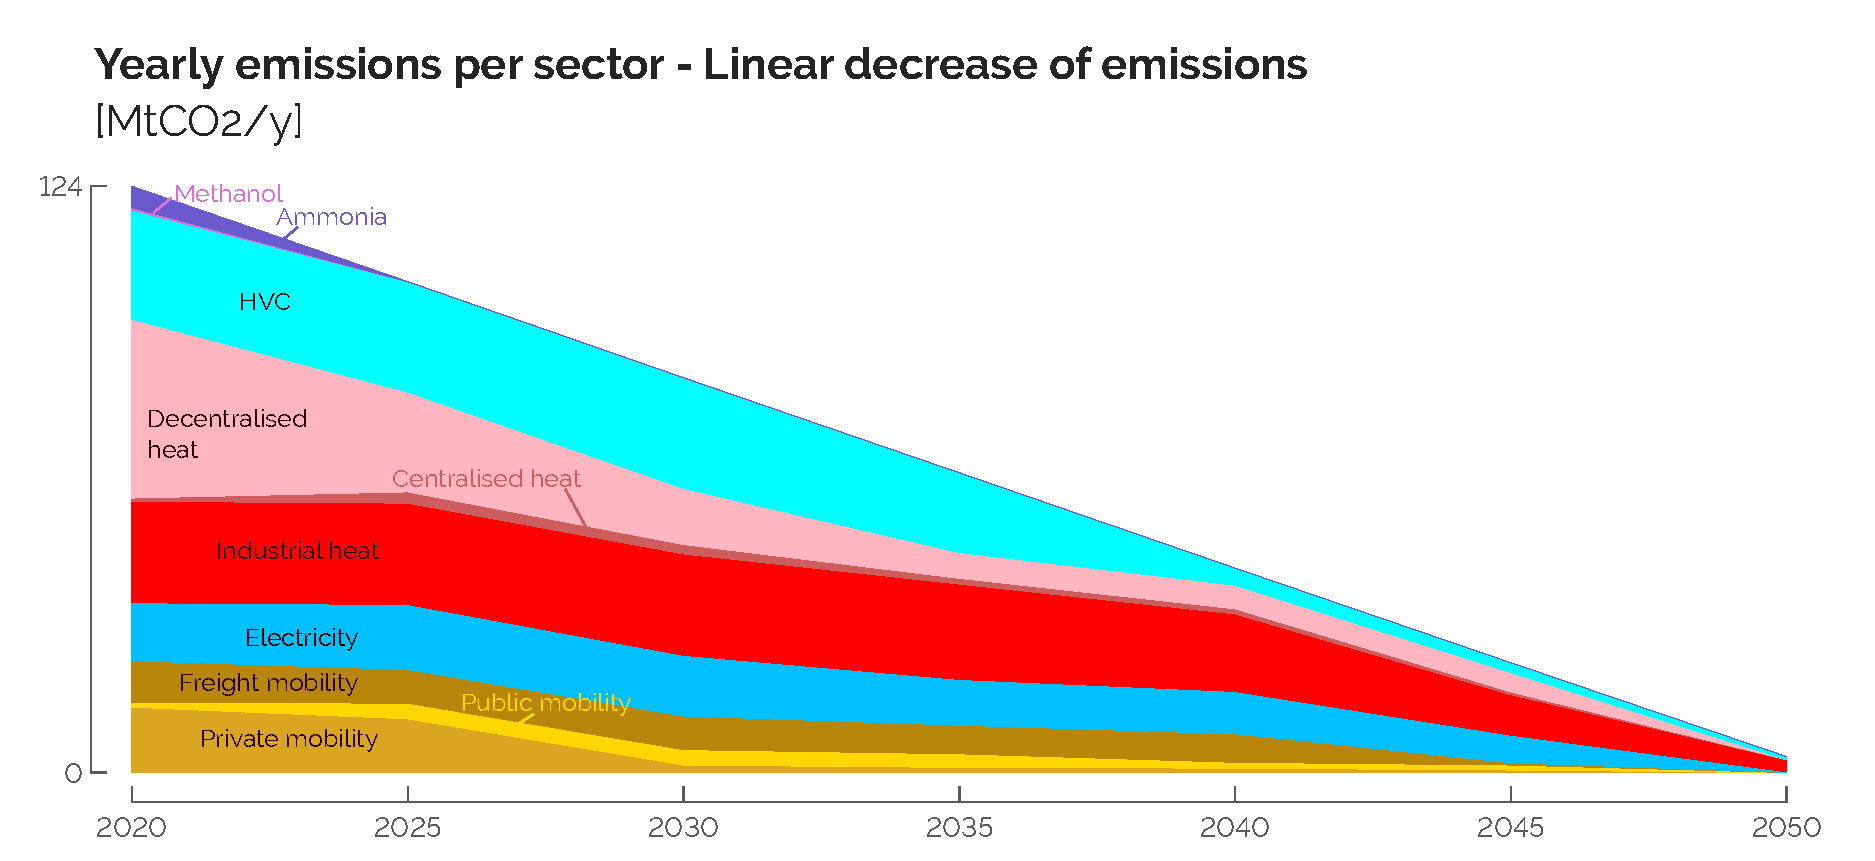
\includegraphics[width=0.49\textwidth]{GWP_per_sector_lin.pdf}
\caption{Respecting the \ce{CO2}-budget imposed in the REF case drastically cuts the emissions of the system, especially in the production of \glsxtrfull{HVC} and the high-temperature heating sector.}
\label{fig:app_CO2_REF_lin}
\end{figure}

\subsection{Comparison without restriction on \gls{GHG}}
\label{app:pfmomy_comparison_without_GHG}

The outcomes of a model could be limited when the case study is too restrictive. Indeed, ones could argue that the comparison between myopic, monthly and perfect foresight are very similar as the energy system is strongly constrained in terms of \gls{GHG} emissions.

In the following, we perform a similar comparison in the transition pathway without restricting the \gls{GHG} emissions. \\

\myparagraph{Reference case}\\

\noindent
Figure \ref{fig:EnergyMixPathwayWithoutGHGLimit} illustrates the transition taken by Belgium without restriction on the \gls{GHG} emissions. 

 \begin{figure}[!htbp]
\centering
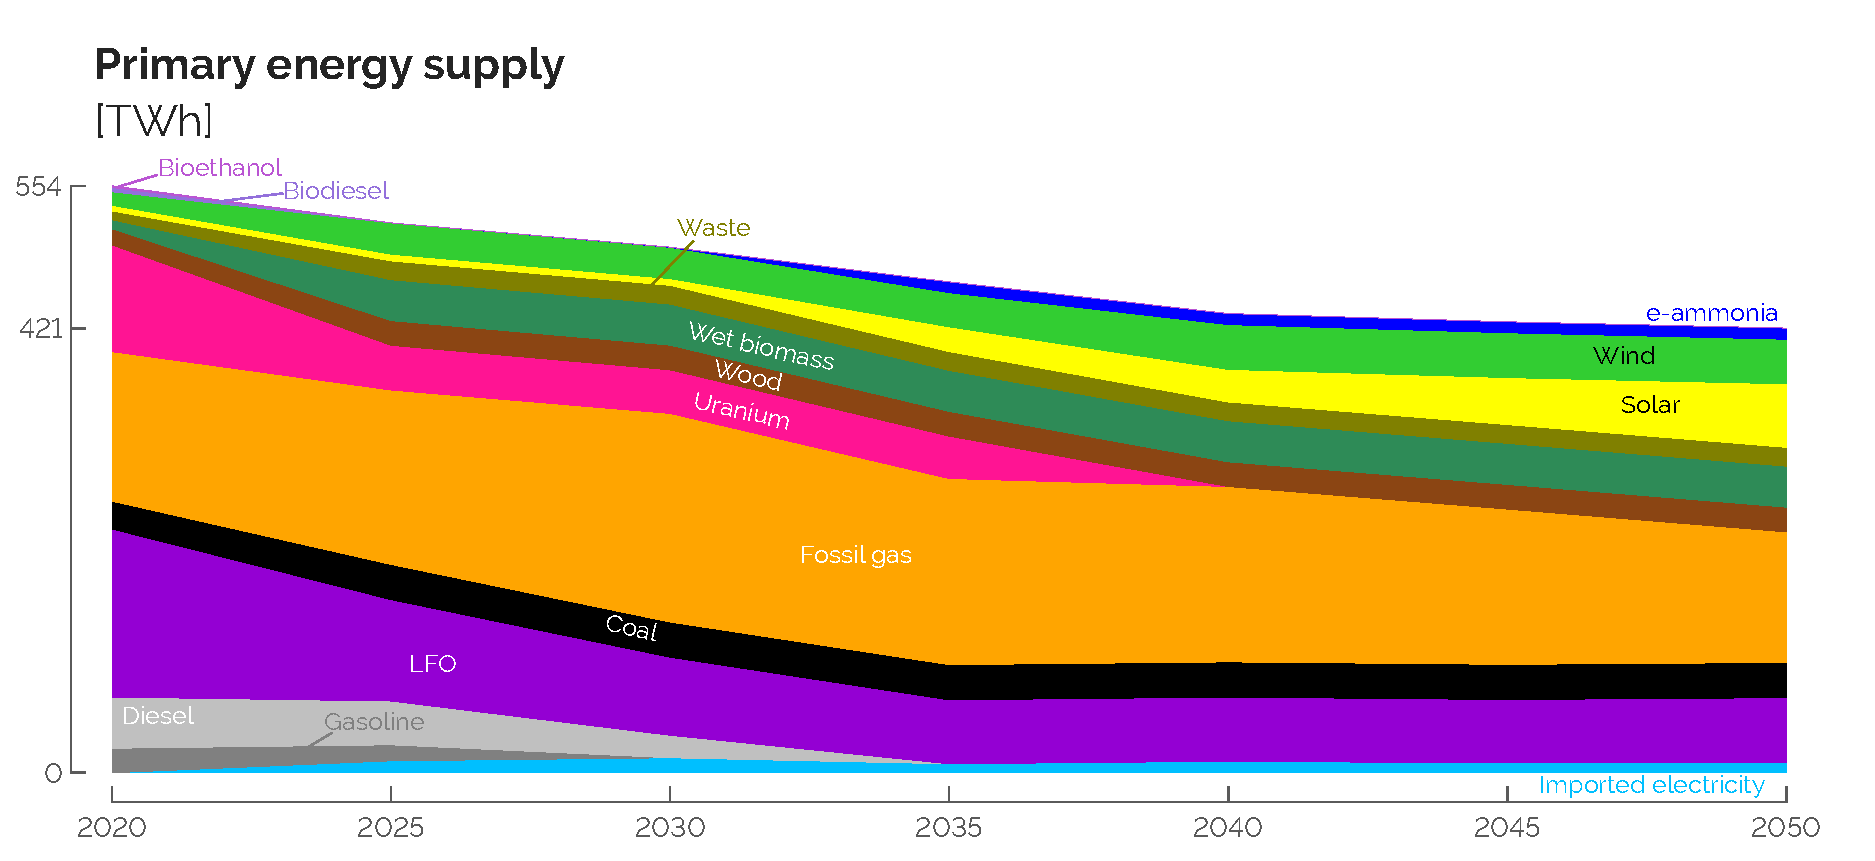
\includegraphics[width=\textwidth]{Resources_no_traj.pdf}
\caption{Primary energy mix of a non-constrained energy transition. In this results, carbon neutrality is not reached in 2050. Some fossil fuels remain used.}
\label{fig:EnergyMixPathwayWithoutGHGLimit}
\end{figure}

Similar trends that for the defossilisation are observed: primary energy mix reduces, renewable energy integration rises and an electro-fuel is imported. However, some changes reflects the cheapest option that the system could utilise to reach a cheaper transition, such as using as little electrofuels as possible. In this case, only e-ammonia is used for its end use demand.

Instead of analysing the energy system in details, the following paragraphs will investigate if the comparison findings are consistent on a different case study.\\

\myparagraph{Comparison with Myopic approach}\\

\noindent
Several key messages of the comparison have been summarised in Table \ref{tab:PF_MY}. In the following paragraph we analyse how these conclusions are affected when the constraint on the \gls{GHG}-emissions trajectory is removed. 

First, considering the overall transition cost, the myopic approach keeps on making short-term savings, \ie down to -0.2\%, before ending up with a more expensive transition by 2050, \ie +0.2\%. Similarly to the case with an imposed \gls{GHG}-emissions trajectory, myopic optimisation invests more, compared to the perfect foresight, at early stages into \gls{VRES} technologies to benefit from the significant salvage values of the related grid infrastructures. In 2030, the salvage value of the infrastructures and electricity-generation technologies account for 80.2 and 56.2 b€\textsubscript{2015}, respectively, whereas the overall CAPEX are 404.8 b€\textsubscript{2015} by then.

Then, in the case with a prescribed \gls{GHG}-emissions trajectory, the myopic approach had to invest more by the end of the transition to renew \gls{PV} installed more massively at early stages and that reached the end of their lifetime before the end of the transition. In the case without this emissions trajectory, there is less an urgency/need for integrating renewables in the system. Consequently, in the latter case, there is not such an extra-investment to make to renew too old renewable assets. On top of this, the slower uprise of \gls{VRES} in the case without emissions trajectory leads to a smaller difference of electrification of the other sectors between the perfect foresight and myopic approaches.

Finally, even though the way to get there differs between the perfect foresight and the myopic approaches, the system designs by 2050 are very similar between these two in most of the sectors. The main observed difference is in the freight transport where diesel boats are preferred to gas boats. This can be looked as a result of the lock-in effect where choices made at early stages, due to the limited foresight, remain in place in the longer term. 

In essence, when comparing perfect foresight and myopic approaches, distinctions arise in minor aspects, while the fundamental conclusions of Table \ref{tab:PF_MY} were verified. These variances have been elucidated in the preceding enumerated points and can primarily be attributed to the changes in the case study, rather than reflecting limitations inherent to the model or the comparative analysis itself.



\section{Uncertainty characterisation for the 5-year steps transition} 
\label{app:UC_full}
Table \ref{tab:UC_full} summarises the uncertainty ranges for the different groups of technologies and resources, for the year 2025. Refer to \cite{Moret2017, Moret2017PhDThesis} for the methodology and sources. As the model optimises the system every 5 years, $N=5$ has been selected to get the final ranges of uncertainties of type II and III, based on the work of \citet{Moret2017PhDThesis}. For type III uncertainties (\ie uncertainty ranges increasing with time), a 50\% increase has been set arbitrarily between the ranges for 2025 and these same ranges for 2050. In other words, for these specific uncertainties, the ranges for 2050 are 50\% larger than for 2025.

\citet{rixhon2021role} analysed the impact of these parameters on the total cost of the snapshot Belgian whole-energy system in 2050 subject to different \gls{GWP} limits. Based on this work, we have selected a subset of impacting uncertainties, added others due to the pathway formulation (\eg $\Delta_{\mathrm{change,pass}}$), and listed them in Table \ref{tab:UC_full}. The uncertainty characterisation gives the uncertainty ranges per parameter or group of parameters (category).

This work considers nine groups of uncertain parameters: (i) the cost of purchasing imported energy carriers; (ii) the investment cost (\ie CAPEX) of some technologies, mostly related to the mobility sector and the integration of renewables; (iii) the maintenance cost (\ie OPEX) of every technology; (iv) the consumption of electric and fuel cells vehicles in the mobility sector; (v) the potential installed capacity of renewables; (vi) the hourly load factor of renewables accounting for variability of solar irradiance or wind speed; (vii) the availability of resources considered as limited (\ie biomass and electricity); (viii) the end-use-demands split per sector of activities (\ie households, services, passenger mobility and industry) and (ix) other parameters like the interest rate or the modal share change in different key sectors. For the specific case of \gls{SMR}, the parameter $f_{\mathrm{max,SMR}}$ will influence the maximum capacity (\ie 6~GW) to install to translate somehow the readiness of this technology. If it is (i) smaller than 0.6, there is no possibility to install \gls{SMR} during the transition; (ii) between 0.6 and 0.8, these 6~GW can be installed only in 2050; (iii) between 0.8 and 0.9, these can be installed from 2045 onward and; (iv) higher than 0.9, the prescribed maximum capacity can be installed from 2040 onward. 

% \textcolor{red}{\textbf{See low-wind speed in 2021 from energy key data edition february 2023 (wind-based production decreased 6.4\% despite additional wind farm installations), to justify the -22\% for c,p,t}}

%$^{(a)}$ Per \cite{Moret2017PhDThesis}, \og I: investment-type, II: operation-type (constant uncertainty over time), III: operation-type (uncertainty increasing over time)\fg. $^{(b)}$ The nominal values of each of the parameters is 0, meaning no variation compared to the nominal values of the impacted parameter in the model. $^{(c)}$ This range has been inferred from the local sensitivity analysis performed by \citet{PATHS2050}.

\begin{table}[htbp!]
\caption{Application of the uncertainty characterization method to the EnergyScope Pathway model for the year 2025. }
\label{tab:UC_full}
\begin{minipage}{\linewidth}
\centering
\resizebox{\textwidth}{!}{
\begin{tabular}{l l l c c c}
\toprule
\multirow{2}{*}{\textbf{Category}} & \multirow{2}{*}{\textbf{Parameter}} & \multirow{2}{*}{\textbf{Meaning}} & \multirow{2}{*}{\textbf{Type}\footnote{\label{foot:type_uncert_range_app}Per \citet{Moret2017PhDThesis}, \og I: investment-type, II: operation-type (constant uncertainty over time), III: operation-type (uncertainty increasing over time)\fg . }}  & \multicolumn{2}{c}{\textbf{Relative variation}\footnote{\label{foot:nom_val_uncert_app}The nominal values of each of the parameters is 0, meaning no variation compared to the nominal values of the impacted parameter in the model. }}\\
    & & & &	 min 	&	 max \\ 	
\midrule		
\multirow{4}{*}{\textbf{Cost of purchasing}} & $c_{\mathrm{op,fossil}}$ & Purchase fossil fuels & II & -64.3\% & 179.8\% \\
& $c_{\mathrm{op,elec}}$ & Purchase electricity & II & -64.3\% & 179.8\% \\
& $c_{\mathrm{op,electrofuels}}$ & Purchase electrofuels & II & -64.3\% & 179.8\% \\
& $c_{\mathrm{op,biofuels}}$ & Purchase biofuels & II & -64.3\% & 179.8\% \\
\midrule
\multirow{9}{*}{\textbf{Investment cost}} &$c_{\mathrm{inv,car}}$ & CAPEX car  & I & -21.6\% & 25.0\% \\
& $c_{\mathrm{inv,bus}}$ & CAPEX bus & I & -21.6\% & 25.0\% \\
& $c_{\mathrm{inv,ic\_prop}}$ & CAPEX ICE & I & -21.6\% & 25.0\% \\
& $c_{\mathrm{inv,e\_prop}}$ & CAPEX electric motor & I & -39.6\% & 39.6\% \\
& $c_{\mathrm{inv,fc\_prop}}$ & CAPEX fuel cell engine & I & -39.6\% & 39.6\% \\
& $c_{\mathrm{inv,efficiency}}$ & CAPEX efficiency measures & I & -39.3\%  & 39.3\% \\
& $c_{\mathrm{inv,PV}}$ & CAPEX PV & I & -39.6\% & 39.6\% \\
& $c_{\mathrm{inv,grid}}$ & CAPEX power grid & I & -39.3\% & 39.3\% \\
& $c_{\mathrm{inv,grid\_enforce}}$ & CAPEX grid reinforcement & I & -39.3\% & 39.3\% \\
& $c_{\mathrm{inv,nuclear\_SMR}}$ & CAPEX \gls{SMR}\footnote{\label{foot:range_SMR_app}This range has been inferred from the local sensitivity analysis performed by \citet{PATHS2050}.} & I & -40.0\% & 44.0\% \\
\midrule
\textbf{Maintenance cost} & $c_{\mathrm{maint,var}}$ & Variable OPEX of technologies & I & -48.2\% & 35.7\% \\
\midrule
\multirow{2}{*}{\textbf{Consumption}} &$\eta_{\mathrm{e\_prop}}$ & Consumption electric vehicles & I & -28.7\% & 28.7\% \\
& $\eta_{\mathrm{fc\_prop}}$ & Consumption fuel cell vehicles & I & -28.7\% & 28.7\% \\
\midrule
\multirow{3}{*}{\textbf{Potential installed capacity}} &$f_{\mathrm{max,PV}}$ & Max capacity PV & I & -24.1\% & 24.1\% \\
& $f_{\mathrm{max,windon}}$ & Max capacity onshore wind & I & -24.1\% & 24.1\% \\
& $f_{\mathrm{max,windoff}}$ & Max capacity offshore wind & I & -24.1\% & 24.1\% \\
\midrule
\multirow{2}{*}{\textbf{Hourly load factor}} & $c_{\mathrm{p,t,PV}}$ & Hourly load factor PV & II & -22.1\% & 22.1\% \\
& $c_{\mathrm{p,t,winds}}$ & Hourly load factor wind turbines & II & -22.1\% & 22.1\% \\
\midrule
\multirow{2}{*}{\textbf{Resource availability}} & $avail_{\mathrm{elec}}$ & Available electricity import & I & -32.1\% & 32.1\% \\
& $avail_{\mathrm{biomass}}$ & Available local biomass & I & -32.1\% & 32.1\% \\
\midrule

\multirow{4}{*}{\textbf{End-use demand}} &$HH\_EUD$ & Households EUD & III & -13.8\% & 11.2\% \\
& $services\_EUD$ & Services EUD & III & -14.3\% & 11\% \\
& $pass\_EUD$ & Passenger mobility EUD & III & -7.5\% & 7.5\% \\
& $industry\_EUD$ & Industry EUD & III & -20.5\% & 16.0\% \\
\midrule

\multirow{6}{*}{\textbf{Miscellaneous}} &$i_{\mathrm{rate}}$  & Interest rate & I & -46.2\% & 46.2\% \\
& $\%_{\mathrm{pub,max}}$ & Max share of public transport & I & -10\% & 10\% \\
& $\Delta_{\mathrm{change,freight}}$ & Modal share change freight mobility & - & -30\% & 30\% \\
& $\Delta_{\mathrm{change,pass}}$ & Modal share change passenger mobility & - & -30\% & 30\% \\
& $\Delta_{\mathrm{change,LT\_heat}}$ & Modal share change LT-heat & - & -30\% & 30\% \\
& $f_{\mathrm{max,SMR}}$ & Potential capacity \gls{SMR} & - & 0 & 1 \\

\bottomrule							

\end{tabular}}
\end{minipage}
\end{table}